\documentclass[a4paper,12pt,twoside]{memoir}

% Castellano
\usepackage[spanish,es-tabla]{babel}
\selectlanguage{spanish}
\usepackage[utf8]{inputenc}
\usepackage[T1]{fontenc}
\usepackage{lmodern} % Scalable font
\usepackage{microtype}
\usepackage{placeins}

\RequirePackage{booktabs}
\RequirePackage[table]{xcolor}
\RequirePackage{xtab}
\RequirePackage{multirow}

% Links
\PassOptionsToPackage{hyphens}{url}\usepackage[colorlinks]{hyperref}
\hypersetup{
	allcolors = {red}
}

% Ecuaciones
\usepackage{amsmath}

% Rutas de fichero / paquete
\newcommand{\ruta}[1]{{\sffamily #1}}

% Párrafos
\nonzeroparskip

% Huérfanas y viudas
\widowpenalty100000
\clubpenalty100000

% Imagenes
\usepackage{graphicx}
\newcommand{\imagen}[2]{
	\begin{figure}[!h]
		\centering
		\includegraphics[width=0.9\textwidth]{#1}
		\caption{#2}\label{fig:#1}
	\end{figure}
	\FloatBarrier
}

\newcommand{\imagenflotante}[2]{
	\begin{figure}%[!h]
		\centering
		\includegraphics[width=0.9\textwidth]{#1}
		\caption{#2}\label{fig:#1}
	\end{figure}
}



% El comando \figura nos permite insertar figuras comodamente, y utilizando
% siempre el mismo formato. Los parametros son:
% 1 -> Porcentaje del ancho de página que ocupará la figura (de 0 a 1)
% 2 --> Fichero de la imagen
% 3 --> Texto a pie de imagen
% 4 --> Etiqueta (label) para referencias
% 5 --> Opciones que queramos pasarle al \includegraphics
% 6 --> Opciones de posicionamiento a pasarle a \begin{figure}
\newcommand{\figuraConPosicion}[6]{%
  \setlength{\anchoFloat}{#1\textwidth}%
  \addtolength{\anchoFloat}{-4\fboxsep}%
  \setlength{\anchoFigura}{\anchoFloat}%
  \begin{figure}[#6]
    \begin{center}%
      \Ovalbox{%
        \begin{minipage}{\anchoFloat}%
          \begin{center}%
            \includegraphics[width=\anchoFigura,#5]{#2}%
            \caption{#3}%
            \label{#4}%
          \end{center}%
        \end{minipage}
      }%
    \end{center}%
  \end{figure}%
}

%
% Comando para incluir imágenes en formato apaisado (sin marco).
\newcommand{\figuraApaisadaSinMarco}[5]{%
  \begin{figure}%
    \begin{center}%
    \includegraphics[angle=90,height=#1\textheight,#5]{#2}%
    \caption{#3}%
    \label{#4}%
    \end{center}%
  \end{figure}%
}
% Para las tablas
\newcommand{\otoprule}{\midrule [\heavyrulewidth]}
%
% Nuevo comando para tablas pequeñas (menos de una página).
\newcommand{\tablaSmall}[5]{%
 \begin{table}
  \begin{center}
   \rowcolors {2}{gray!35}{}
   \begin{tabular}{#2}
    \toprule
    #4
    \otoprule
    #5
    \bottomrule
   \end{tabular}
   \caption{#1}
   \label{tabla:#3}
  \end{center}
 \end{table}
}

%
% Nuevo comando para tablas pequeñas (menos de una página).
\newcommand{\tablaSmallSinColores}[5]{%
 \begin{table}[H]
  \begin{center}
   \begin{tabular}{#2}
    \toprule
    #4
    \otoprule
    #5
    \bottomrule
   \end{tabular}
   \caption{#1}
   \label{tabla:#3}
  \end{center}
 \end{table}
}

\newcommand{\tablaApaisadaSmall}[5]{%
\begin{landscape}
  \begin{table}
   \begin{center}
    \rowcolors {2}{gray!35}{}
    \begin{tabular}{#2}
     \toprule
     #4
     \otoprule
     #5
     \bottomrule
    \end{tabular}
    \caption{#1}
    \label{tabla:#3}
   \end{center}
  \end{table}
\end{landscape}
}

%
% Nuevo comando para tablas grandes con cabecera y filas alternas coloreadas en gris.
\newcommand{\tabla}[6]{%
  \begin{center}
    \tablefirsthead{
      \toprule
      #5
      \otoprule
    }
    \tablehead{
      \multicolumn{#3}{l}{\small\sl continúa desde la página anterior}\\
      \toprule
      #5
      \otoprule
    }
    \tabletail{
      \hline
      \multicolumn{#3}{r}{\small\sl continúa en la página siguiente}\\
    }
    \tablelasttail{
      \hline
    }
    \bottomcaption{#1}
    \rowcolors {2}{gray!35}{}
    \begin{xtabular}{#2}
      #6
      \bottomrule
    \end{xtabular}
    \label{tabla:#4}
  \end{center}
}

%
% Nuevo comando para tablas grandes con cabecera.
\newcommand{\tablaSinColores}[6]{%
  \begin{center}
    \tablefirsthead{
      \toprule
      #5
      \otoprule
    }
    \tablehead{
      \multicolumn{#3}{l}{\small\sl continúa desde la página anterior}\\
      \toprule
      #5
      \otoprule
    }
    \tabletail{
      \hline
      \multicolumn{#3}{r}{\small\sl continúa en la página siguiente}\\
    }
    \tablelasttail{
      \hline
    }
    \bottomcaption{#1}
    \begin{xtabular}{#2}
      #6
      \bottomrule
    \end{xtabular}
    \label{tabla:#4}
  \end{center}
}

%
% Nuevo comando para tablas grandes sin cabecera.
\newcommand{\tablaSinCabecera}[5]{%
  \begin{center}
    \tablefirsthead{
      \toprule
    }
    \tablehead{
      \multicolumn{#3}{l}{\small\sl continúa desde la página anterior}\\
      \hline
    }
    \tabletail{
      \hline
      \multicolumn{#3}{r}{\small\sl continúa en la página siguiente}\\
    }
    \tablelasttail{
      \hline
    }
    \bottomcaption{#1}
  \begin{xtabular}{#2}
    #5
   \bottomrule
  \end{xtabular}
  \label{tabla:#4}
  \end{center}
}



\definecolor{cgoLight}{HTML}{EEEEEE}
\definecolor{cgoExtralight}{HTML}{FFFFFF}

%
% Nuevo comando para tablas grandes sin cabecera.
\newcommand{\tablaSinCabeceraConBandas}[5]{%
  \begin{center}
    \tablefirsthead{
      \toprule
    }
    \tablehead{
      \multicolumn{#3}{l}{\small\sl continúa desde la página anterior}\\
      \hline
    }
    \tabletail{
      \hline
      \multicolumn{#3}{r}{\small\sl continúa en la página siguiente}\\
    }
    \tablelasttail{
      \hline
    }
    \bottomcaption{#1}
    \rowcolors[]{1}{cgoExtralight}{cgoLight}

  \begin{xtabular}{#2}
    #5
   \bottomrule
  \end{xtabular}
  \label{tabla:#4}
  \end{center}
}



\graphicspath{ {./img/} }

% Capítulos
\chapterstyle{bianchi}
\newcommand{\capitulo}[2]{
	\setcounter{chapter}{#1}
	\setcounter{section}{0}
	\setcounter{figure}{0}
	\setcounter{table}{0}
	\chapter*{#2}
	\addcontentsline{toc}{chapter}{#2}
	\markboth{#2}{#2}
}

% Apéndices
\renewcommand{\appendixname}{Apéndice}
\renewcommand*\cftappendixname{\appendixname}

\newcommand{\apendice}[1]{
	%\renewcommand{\thechapter}{A}
	\chapter{#1}
}

\renewcommand*\cftappendixname{\appendixname\ }

% Formato de portada
\makeatletter
\usepackage{xcolor}
\newcommand{\tutor}[1]{\def\@tutor{#1}}
\newcommand{\course}[1]{\def\@course{#1}}
\definecolor{cpardoBox}{HTML}{E6E6FF}
\def\maketitle{
  \null
  \thispagestyle{empty}
  % Cabecera ----------------
\noindent
\includegraphics[width=\textwidth]{cabecera}\vspace{1cm}%
  \vfill
  % Título proyecto y escudo informática ----------------
  \colorbox{cpardoBox}{%
    \begin{minipage}{.8\textwidth}
      \vspace{.5cm}\Large
      \begin{center}
      \textbf{TFG del Grado en Ingeniería Informática}\vspace{.6cm}\\
      \textbf{\LARGE\@title{}}
      \end{center}
      \vspace{.2cm}
    \end{minipage}

  }%
  \hfill\begin{minipage}{.20\textwidth}
    
\includegraphics[width=\textwidth]{escudoInfor}
  \end{minipage}
  \vfill
  % Datos de alumno, curso y tutores ------------------
  \begin{center}%
  {%
    \noindent\LARGE
    Presentado por \@author{}\\ 
    Universidad de Burgos \\ \@date{}\\
    Tutor: \@tutor{}\\
  }%
  \end{center}%
  \null
  \cleardoublepage
  }
\makeatother

\newcommand{\nombre}{Joaquín García Molina} %%% cambio de comando

% Datos de portada
\title{GII\_O\_MA\_19.07 \\Comparador de métricas de evolución en repositorios Software}
\author{\nombre}
\tutor{Carlos López Nozal}
\date{\today}



\begin{document}

% Otras variables para la memoria
\newcommand{\dniAlumno}{76441581-T}
\newcommand{\titulo}{GII\_O\_MA\_19.07 \\Comparador de métricas de evolución en repositorios Software}
\newcommand{\tutorPrincipal}{Carlos López Nozal}

\maketitle


\newpage\null\thispagestyle{empty}\newpage


%%%%%%%%%%%%%%%%%%%%%%%%%%%%%%%%%%%%%%%%%%%%%%%%%%%%%%%%%%%%%%%%%%%%%%%%%%%%%%%%%%%%%%%%
\thispagestyle{empty}


\noindent
\includegraphics[width=\textwidth]{cabecera}\vspace{1cm}

\noindent D. \tutorPrincipal, profesor del departamento de nombre departamento, área de nombre área.

\noindent Expone:

\noindent Que el alumno D. \nombre, con DNI \dniAlumno, ha realizado el Trabajo final de Grado en Ingeniería Informática titulado \titulo. 

\noindent Y que dicho trabajo ha sido realizado por el alumno bajo la dirección del que suscribe, en virtud de lo cual se autoriza su presentación y defensa.

\begin{center} %\large
En Burgos, {\large \today}
\end{center}

\vfill\vfill\vfill

% Author and supervisor
\begin{minipage}{0.45\textwidth}
\begin{flushleft} %\large
Vº. Bº. del Tutor:\\[2cm]
D. \tutorPrincipal
\end{flushleft}
\end{minipage}
\hfill
\begin{minipage}{0.45\textwidth}

\end{minipage}
\hfill

\vfill

% para casos con solo un tutor comentar lo anterior
% y descomentar lo siguiente
%Vº. Bº. del Tutor:\\[2cm]
%D. nombre tutor


\newpage\null\thispagestyle{empty}\newpage




\frontmatter

% Abstract en castellano
\renewcommand*\abstractname{Resumen}
\begin{abstract}

Este TFG desarrolla una segunda iteración sobre \textit{\textbf{Evolution Metrics Gauge}}, un software para calcular métricas de evolución del proceso de desarrollo y obtenidas de la interacción de los desarrolladores en sus repositorios de \textit{Gitlab}.
\textit{Evolution Metrics Gauge} es una aplicación web escrita en \textit{Java} con el framework \textit{Vaddin}. Toma como entrada un conjunto de repositorios públicos o privados y calcula métricas de evolución que permiten comparar los proyectos. 

El objetivo de este TFG es realizar un incremento funcional aplicando el flujo de desarrollo y despliegue continuo. En concreto, se actualizará y probará el desarrollo con una nueva versión de \textit{Vaadin}. En el incremento se realizará la integración necesaria para poder trabajar con la plataforma \textit{GitHub}, se integrará con la funcionalidad previa y se añadirán nuevas métricas a las ya existentes para trabajar con ellas y con las ya existentes con proyectos procedentes de ambas forjas de repositorios.   
Gracias a esto, este TFG proporciona una herramienta que ayuda a poder gestionar la calidad de los procesos de desarrollo con independencia de la forja utilizada, ya sea \textit{GitHub} o \textit{GitLab}, ya que gracias a éste podremos obtener y evaluar las diferentes métricas de los repositorios y con ellas evaluar el proceso de desarrollo de los mismos.

%Repositorio del proyecto:
%\url{https://github.com/Joaquin-GM/GII_O_MA_19.07-Comparador-de-metricas-de-evolucion-en-repositorios-Software}


\end{abstract}

\renewcommand*\abstractname{Descriptores}
\begin{abstract}
Métricas de evolución, proceso de desarrollo de software, gestión de calidad, repositorios de código, \textit{GitLab}, \textit{GitHub}, comparación de proyectos software, aplicaciones web.
\end{abstract}

\newpage
% Abstract en inglés
\renewcommand*\abstractname{Abstract}
\begin{abstract}

This TFG develops a second iteration on \textit{\textbf{Evolution Metrics Gauge}}, a software to calculate evolution metrics of the development process and obtained from the interaction of developers in their Gitlab repositories.
Evolution Metrics Gauge is a web application written in \textit{Java} with the \textit{Vaddin} framework. It takes as input a set of public or private repositories and calculates evolution metrics that allow projects to be compared.

The objective of this \textit{TFG} is to carry out a functional increase by applying the flow of development and continuous use defined. Specifically, development will be updated and tested with a new version of \textit{Vaadin}. In the increment, the integration with \textit{GitHub} will be achieved and it will be integrated with the existing functionality and also new metrics will be added to the existing ones to work with them with repositories from both sources.
Thanks to this, this \textit{TFG} brings a tool that helps to manage the quality of the development processes regardless of the forge used, whether it is \textit{GitHub} or \textit{GitLab}, because thanks to the project we will be able to obtain and evaluate different metrics from the repositories and with them evaluate the development proccess of the repositories.

%Project repository:
%\url{https://github.com/Joaquin-GM/GII_O_MA_19.07-Comparador-de-metricas-de-evolucion-en-repositorios-Software}

\end{abstract}

\renewcommand*\abstractname{Keywords}
\begin{abstract}
Evolution metrics, software development process,quality management, code repositories, GitLab, GitHub, comparison of software projects, web applications.
\end{abstract}

\clearpage

% Indices
\tableofcontents

\clearpage

\listoffigures

\clearpage

\listoftables
\clearpage

\mainmatter
\capitulo{1}{Introducción}

% Descripción del contenido del trabajo y del estructura de la memoria y del resto de materiales entregados.

El desarrollo de software es una actividad que puede ser enormemente compleja al poder desarrollar proyectos de gran envergadura que impliquen a muchas personas y entidades trabajando con diferentes herramientas y con variados patrones de organización \cite{jacobson_proceso_2000}. Esta complejidad existe a nivel técnico ya que se requiere que se cumplan los requisitos establecidos funcionales pero es necesario que también se cumpla con los no funcionales como pueden ser la seguridad, la posibilidad de actualización, la escalabilidad de la arquitectura elegida, los tiempos de carga, etc.
Además, esta complejidad existe también a nivel organizativo, es necesario que los jefes de proyecto sean capaces de organizar a los equipos y el trabajo a realizar de forma que se optimice tanto el tiempo como los recursos económicos disponibles.

Para poder salvar esta complejidad y que los jefes de proyecto sean capaces de llevar a cabo su tarea de optimización de los recursos se han creado diferentes modelos que permiten definir las actividades y tareas realizadas en los proyectos de forma organizada y lo más sencilla posible. Entre estos modelos destaca \textit{\textbf{Unified Process (UP)}} \cite{jacobson_proceso_2000} donde se definen las siguientes tareas en un proyecto: 

\begin{itemize}
	\item Captura de requisitos.
	\item Análisis
	\item Diseño
	\item Implementación
	\item Prueba
\end{itemize}

Estas diferentes tareas o fases de realizan de forma iterativa e incremental, es decir, tras la fase de prueba se comprueba que no existen nuevos requisitos y se repite todo el proceso. Cada una de estas iteraciones ha de resultar en un entregable o artefacto a ser posible funcional.

Este desarrollo iterativo incremental está también reflejado en otras metodologías de trabajo como son las de desarrollo ágil como Scrum, Lean o eXtreme Programming.


Para poder llevar a cabo este desarrollo iterativo y de forma colaborativa, entre varios desarrolladores, es necesario disponer de herramientas que permitan la gestión de los productos software como el proceso de desarrollo del equipo. Estas herramientas son los repositorios de software que son espacios centralizados donde se almacena, organiza, mantiene y difunde información digital, habitualmente archivos informáticos, que pueden contener trabajos científicos, conjuntos de datos o software\footnote{\url{https://es.wikipedia.org/}}. 

Las herramientas de control de repositorios o forjas de proyectos software han evolucionado con los años y tienen muchas más funcionalidades, además del control de cambios de los archivos, se centran en fomentar el desarrollo colaborativo y la interacción entre desarrolladores.
Entre dichas funcionalidades podemos nombrar el control de versiones, el control de los archivos de forma colaborativa, almacenándose tanto los propios archivos como las interacciones entre los miembros del equipo que los manipulan, sistemas de revisión de calidad, sistemas de control de incidencias (o \textit{issues}) o sistemas de integración y despliegue continuo denominados CI/CD ("Continuous delivery - Continuous deployment").
Entre estas herramientas podemos destacar en la actualidad por ser las más usadas:  GitHub\footnote{\url{https://github.com/}}, GitLab\footnote{\url{https://about.gitlab.com/}} o Bitbucket\footnote{\url{https://bitbucket.org/}}) aunque existen otras como SourceForge\footnote{\url{https://sourceforge.net/}}.

Estas herramientas están en continua evolución desarrollando nuevas funcionalidades para mejorar la experiencia de los desarrolladores y los gestores de proyectos y permiten integración con terceros para ofrecer aquellas características que aún no ofrecen.
En el orden de las metodologías ágiles las diferentes plataformas están avanzando mucho ofreciendo por ejemplo GitLab el módulo GitLab Issues\footnote{\url{https://docs.gitlab.com/ee/user/project/issues/}}) o  
GitHub GitHub Issues\footnote{\url{https://docs.github.com/en/issues/tracking-your-work-with-issues/about-issues}} (mejorado con ZenHub\footnote{\url{https://www.zenhub.com/}}).

Estas herramientas generan una enorme cantidad de información de los proyectos y del proceso de desarrollo. En la actualidad uno de los aspectos del desarrollo de software que más interés despierta y en el que se realizan más avances es en la gestión de esta información ya que, cuanto más se optimice dicha gestión de la información, antes se pueden detectar los fallos en el proceso de desarrollo para optimizarlo.
Este es el campo de trabajo de los jefes de proyecto, el correcto control sobre el proceso de desarrollo y el producto creado. Es por esto crucial que exista una manera de medir si se está realizando correctamente dicho proceso o no.
Para ello existen las control y de predicción \cite{sommerville_ingenierisoftware_2002}. Las primeras se refieren al proceso de desarrollo, y las segundas al producto, en el presente TFG nos centraremos fundamentalmente en las primeras.

Es claro que el resultado de un proyecto dependerá del proceso de desarrollo seguido y su calidad. Esto es explicado, por ejemplo, por Sommerville en \textit{Ingeniería de software} \cite{sommerville_ingenierisoftware_2002} y que cuanto mejor sea este proceso mejores resultados se obtendrán a la finalización de los proyectos.

Este presente TFG pretende profundizar en este punto, mejorar la calidad de los procesos de desarrollo,  implementado medidas automáticas del proceso desarrollado en GitHub. Se implementa una nueva iteración sobre \textit{\textbf{Evolution Metrics Gauge}}, un software para calcular métricas de control\footnote{También llamadas métricas de proceso o métricas de evolución.}.
Dicho software ha sido desarrollado en un TFG previo titulado \textit{\textbf{Evolution Metrics Gauge - Comparador de métricas de evolución en repositorios software}} \cite{TFGPrevio}. Este software consiste en una aplicación Web escrita en lenguaje Java que toma como entrada un conjunto de repositorios públicos o privados de GitLab y calcula métricas de evolución que permiten comparar los proyectos.
En esta nueva iteración se pretende extender la funcionalidad a repositorios de GitHub, añadir otras métricas e implementar diferentes mejoras.




\section{Estructura de la memoria}

La presente memoria tiene la siguiente estructura\footnote{Se parte de lap lantilla LaTex proporcionada en \url{https://github.com/ubutfgm/plantillaLatex}}:

\begin{description}
	\tightlist
	\item[Introducción.] Introducción. Estructura de la memoria y anexos.
	\item[Objetivos del proyecto.] Objetivos que busca alcanzar el proyecto.
	\item[Conceptos teóricos.] Definiciones de los conceptos empleados en el proyecto.
	\item[Técnicas y herramientas.] Técnicas y herramientas utilizadas durante el desarrollo del proyecto.
	\item[Aspectos relevantes del desarrollo.] Aspectos destacables durante el proceso de desarrollo del proyecto.
	\item[Trabajos relacionados y \textit{debt process}.] Desarrollos relacionados y deuda técnica asociada a proceso.
	\item[Conclusiones y líneas de trabajo futuras.] Conclusiones tras la realización del proyecto y posibilidades de mejora o expansión.
\end{description}

Se incluyen también los siguientes anexos:

\begin{description}
	\tightlist
	\item[Plan del proyecto software.] Planificación temporal y estudio de la viabilidad del proyecto.
	\item[Especificación de requisitos del software.] Análisis de los requisitos.
	\item[Especificación de diseño.] Diseño de los datos, diseño procedimental y diseño arquitectónico.
	\item[Manual del programador.] Aspectos relevantes del código fuente.
	\item[Manual de usuario.] Manual de uso para usuarios que utilicen la aplicación.
\end{description}

\capitulo{2}{Objetivos del proyecto}

% Este apartado explica de forma precisa y concisa cuales son los objetivos que se persiguen con la realización del proyecto. Se puede distinguir entre los objetivos marcados por los requisitos del software a construir y los objetivos de carácter técnico que plantea a la hora de llevar a la práctica el proyecto.

El software desarrollado en este TFG, que se encuentra disponible en:\\
\url{https://github.com/Joaquin-GM/GII_O_MA_19.07-Comparador-de-metricas-de-evolucion-en-repositorios-Software}

es una segunda iteración del software desarrollado \textit{\textbf{Evolution Metrics Gauge}}, disponible en: \\
\url{https://gitlab.com/mlb0029/comparador-de-metricas-de-evolucion-en-repositorios-software}
  
Para facilitar la comprensión se divide en esta sección con los objetivos definidos en cada iteración. Además se ha diferenciado entre objetivos generales y técnicos.

\section{Objetivos Evolution Metrics Gauge iteración 1}
A continuación se enumeran los objetivos iniciales de la aplicación ya desarrollada y cómo se han desarrollado: \cite{TFGPrevio}
\begin{itemize}
	\tightlist
	\item Se obtienen medidas de métricas de evolución de uno o varios proyectos alojados en repositorios de \textit{GitLab}.
	\item Las métricas que se calculan de un repositorio  son algunas de las especificadas en la tesis titulada ``\textit{sPACE: Software Project Assessment in the Course of Evolution}'' \cite{ratzinger_space:_2007} y 
	adaptadas a los repositorios software:
	\begin{itemize}
		\tightlist
		\item Número total de incidencias (\textit{issues})
		\item Cambios (\textit{commits}) por incidencia
		\item Porcentaje de incidencias cerrados
		\item Media de días en cerrar una incidencia
		\item Media de días entre cambios
		\item Días entre primer y último cambio
		\item Rango de actividad de cambios por mes
		\item Porcentaje de pico de cambios
	\end{itemize}
	\item Se permite comparar con otros proyectos de la misma naturaleza. Para ello se establecen unos valores umbrales por cada métrica basados en el cálculo de los cuartiles Q1 y Q3. Además, estos valores se calculan dinámicamente y se almacenan en perfiles de configuración de métricas.
	\item Se permite la posibilidad de almacenar de manera persistente estos perfiles de configuración de métricas por medio de archivos para permitir comparaciones futuras.
	\item También se permite almacenar de forma persistente las métricas obtenidas de los repositorios para su posterior consulta o tratamiento. Esto permite comparar nuevos proyectos con proyectos de los que ya se han calculado sus métricas.
	 Esta funcionalidad se basa en la exportación e importación de los valores de métricas obtenidos por la aplicación en diferentes análisis usando archivos \textit{CSV}.
\end{itemize}


\section{Objetivos Evolution Metrics Gauge iteración 2}
   
El objetivo principal del presente TFG es realizar mejoras y extender la funcionalidad que tiene el software \textit{\textbf{Evolution Metrics Gauge}}, un software para calcular métricas de control \footnote{También llamadas métricas de proceso o métricas de evolución} sobre distintos repositorios.
En esta nueva iteración se pretende:

\begin{itemize}
	\tightlist
	\item Calcular las 8 métricas de evolución definidas sobre repositorios \textit{GitHub} además de \textit{GitLab} .
	\item Implementar nuevas métricas a las ya evaluadas.
	\item Realizar pruebas con repositorios de \textit{GitLab} y \textit{GitHub} simultáneamente.
	\item Diseñar una interfaz gráfica que permita la interacción simultánea con repositorios de \textit{GitLab} y \textit{GitHub}.
	\item Comprender y aplicar el flujo de trabajo de integración continua e implementarlo en el proyecto.
	\item Definir un conjunto de pruebas que ayuden a detectar errores de la versión actual y en la nueva funcionalidad.
\end{itemize}

\newpage


\section{Objetivos técnicos}
Este apartado recoge los requisitos técnicos del proyecto existente \cite{TFGPrevio}:
\begin{itemize}
	\tightlist
	\item Diseño de la aplicación de manera que se puedan extender con nuevas métricas con el menor coste de mantenimiento posible. Para ello, se aplica un diseño basado en frameworks y en patrones de diseño \cite{gamma_patrones_2002}.
	\item El diseño de la aplicación facilita la extensión a otras plataformas de desarrollo colaborativo como \textit{GitHub} o \textit{Bitbucket}.
	\item Aplicación del \textit{frameworks `modelo-vista-controlador'} para separar la lógica de la aplicación y la interfaz de usuario.
	\item Creación una batería de pruebas automáticas en los subsistemas de lógica de la aplicación.
	\item Utilización una plataforma de desarrollo colaborativo que incluya un sistema de control de versiones, un sistema de seguimiento de incidencias y que permita una comunicación fluida entre el tutor y el alumno.
	\item Utilización un sistema de integración y despliegue continuo.
	\item Correcta gestión de errores definiendo excepciones de biblioteca y registrando eventos de error e información en ficheros de \textit{log}. 
	\item Aplicar nuevas estructuras  del lenguaje Java para el desarrollo, como son expresiones lambda. 
	\item Utilización de sistemas que aseguren la calidad continua del código que permitan evaluar la deuda técnica del proyecto.
	\item Pruebas la aplicación con ejemplos reales y utilizando técnicas avanzadas, como entrada de datos de test en ficheros con formato tabulado tipo \textit{CSV} (\textit{comma separated values}).
	\item Comprender y aplicar el flujo de trabajo de integración continua del proyecto actual.
	\item Implementar un sistema de registro de errores persistente para gestionar su posible resolución.
	\item Pruebas la aplicación con ejemplos reales y utilizando técnicas avanzadas, como entrada de datos de test en ficheros con formato tabulado tipo \textit{CSV} (\textit{comma separated values}) también para métricas obtenidas de repositorios de \textit{GitHub}. 		
\end{itemize}


%\section{Objetivos técnicos Evolution Metrics Gauge iteración 1}
%\section{Objetivos técnicos Evolution Metrics Gauge iteración 2}
%Además de mantener todos los objetivos técnicos previos fijados para el desarrollo de la aplicación en la primera iteración, se busca profundizar en ellos y mejorar el desarrollo actual. Para ello se se proponen los siguientes objetivos:
%\begin{itemize}
%	\tightlist
%	\item Comprender y aplicar el flujo de trabajo de integración continua del proyecto actual.
%	\item Implementar un sistema de registro de errores persistente para gestionar su posible resolución.
%	\item Pruebas la aplicación con ejemplos reales y utilizando técnicas avanzadas, como entrada de datos de test en ficheros con formato tabulado tipo \textit{CSV} (\textit{comma separated values}) también para métricas obtenidas de repositorios de \textit{GitHub}. 	
%\end{itemize}

\capitulo{3}{Conceptos teóricos}

%En aquellos proyectos que necesiten para su comprensión y desarrollo de unos conceptos teóricos de una determinada materia o de un determinado dominio de conocimiento, debe existir un apartado que sintetice dichos conceptos.
%
%Algunos conceptos teóricos de \LaTeX \footnote{Créditos a los proyectos de Álvaro López Cantero: Configurador de Presupuestos y Roberto Izquierdo Amo: PLQuiz}.
%
%\section{Secciones}
%
%Las secciones se incluyen con el comando section.
%
%\subsection{Subsecciones}
%
%Además de secciones tenemos subsecciones.
%
%\subsubsection{Subsubsecciones}
%
%Y subsecciones. 
%
%
%\section{Referencias}
%
%Las referencias se incluyen en el texto usando cite \cite{wiki:latex}. Para citar webs, artículos o libros \cite{koza92}.
%
%
%\section{Imágenes}
%
%Se pueden incluir imágenes con los comandos standard de \LaTeX, pero esta plantilla dispone de comandos propios como por ejemplo el siguiente:
%
%\imagen{escudoInfor}{Autómata para una expresión vacía}
%
%
%
%\section{Listas de items}
%
%Existen tres posibilidades:
%
%\begin{itemize}
%	\item primer item.
%	\item segundo item.
%\end{itemize}
%
%\begin{enumerate}
%	\item primer item.
%	\item segundo item.
%\end{enumerate}
%
%\begin{description}
%	\item[Primer item] más información sobre el primer item.
%	\item[Segundo item] más información sobre el segundo item.
%\end{description}
%	
%\begin{itemize}
%\item 
%\end{itemize}
%
%\section{Tablas}
%
%Igualmente se pueden usar los comandos específicos de \LaTeX o bien usar alguno de los comandos de la plantilla.
%
%\tablaSmall{Herramientas y tecnologías utilizadas en cada parte del proyecto}{l c c c c}{herramientasportipodeuso}
%{ \multicolumn{1}{l}{Herramientas} & App AngularJS & API REST & BD & Memoria \\}{ 
%HTML5 & X & & &\\
%CSS3 & X & & &\\
%BOOTSTRAP & X & & &\\
%JavaScript & X & & &\\
%AngularJS & X & & &\\
%Bower & X & & &\\
%PHP & & X & &\\
%Karma + Jasmine & X & & &\\
%Slim framework & & X & &\\
%Idiorm & & X & &\\
%Composer & & X & &\\
%JSON & X & X & &\\
%PhpStorm & X & X & &\\
%MySQL & & & X &\\
%PhpMyAdmin & & & X &\\
%Git + BitBucket & X & X & X & X\\
%Mik\TeX{} & & & & X\\
%\TeX{}Maker & & & & X\\
%Astah & & & & X\\
%Balsamiq Mockups & X & & &\\
%VersionOne & X & X & X & X\\
%} 


\section{Evolución de software: Proceso o ciclo de vida de un proyecto software}

Un proceso del software es un conjunto de actividades cuya meta es el desarrollo de software desde cero o la evolución de sistemas software existentes. Para representar este proceso se utilizan modelos de procesos, que no son más que representaciones abstractas de este proceso desde una perspectiva particular. Estos modelos son estrategias para definir y organizar las diferentes actividades y artefactos del proceso. Los artefactos son las salidas de las actividades y el conjunto de artefactos conforman el producto software. Actividades comunes a cualquier modelo son:
\begin{description}
	\item[-- Especificación:] En esta actividad se define la funcionalidad del software y los requerimientos que ha de cumplir.
	\item[-- Diseño e implementación:] En esta fase se define el diseño del software, se generan los artefactos y se realizan pruebas sobre ellos.
	\item[-- Validación:] En esta fase se debe asegurar que los artefactos generados cumplen con su especificación.
	\item[-- Evolución:] Fase asociada a la \textbf{corrección} de defectos o fallos, \textbf{adaptación} del software a cambios en el entorno en el que se utiliza, \textbf{mejora} y ampliación, y \textbf{prevención} mediante técnicas de ingeniería inversa y reingeniería como la refactorización.
\end{description}

Existen modelos de proceso generales como el tradicional modelo en cascada de los 80 (ver Fig. \ref{fig:M3_Modelo_Cascada}) o el modelo incremental (ver Fig. \ref{fig:M3_Scrum}) recogido en métodos y buenas prácticas del desarrollo ágil \cite{scrum_master_scrum_2019} como \textit{Scrum, eXtreme Programming} o \textit{Lean} entre otros. En el caso de  \textit{Unified Process} (\textit{UP}) \cite{jacobson_proceso_2000} se identifican las siguientes actividades o flujos de trabajo: recolección de requisitos, diseño e implementación, pruebas y despliegue. Además, en \textit{UP} se añaden tres flujos de trabajo de soporte: configuración de cambios, gestión de proyecto y gestión de entorno. Estos flujos de trabajo se aplican iterativamente durante varias fases del desarrollo en cada una de las cuales se incrementa el producto software con algún artefacto resultado de la actividad.

\begin{figure}[!h]
	\centering
	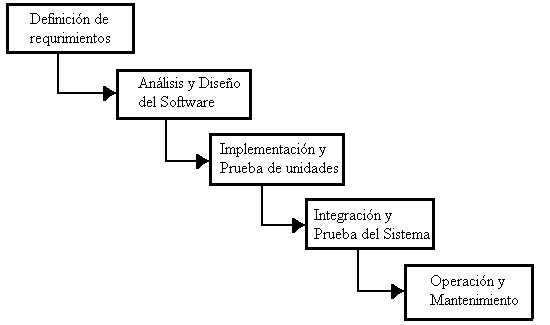
\includegraphics[scale=0.65]{M3_Modelo_Cascada}
	\caption{Modelo de proceso en cascada \cite{wikipedia_software_2019}}
	\label{fig:M3_Modelo_Cascada}
\end{figure}
\FloatBarrier

\begin{figure}[!h]
	\centering
	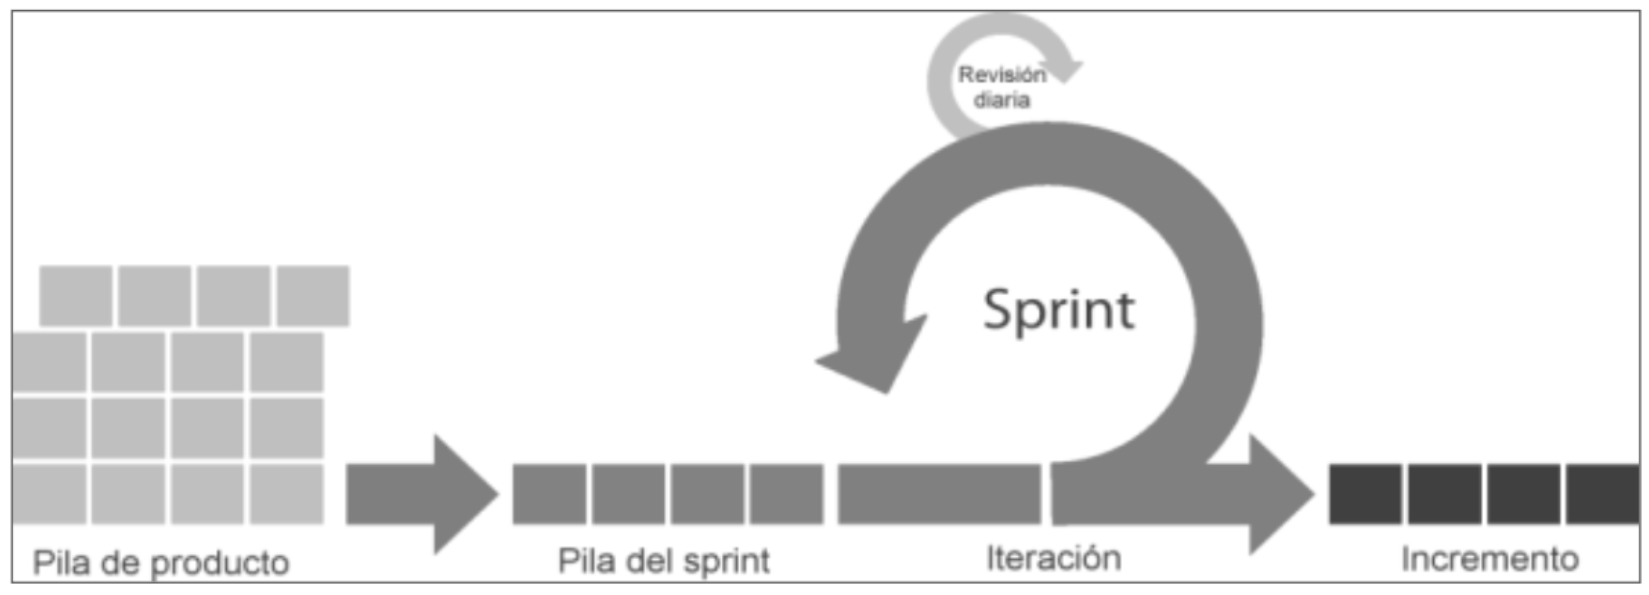
\includegraphics[scale=0.30]{M3_Scrum}
	\caption{Modelo de proceso incremental: \textit{Scrum} \cite{scrum_master_scrum_2019}}
	\label{fig:M3_Scrum}
\end{figure}
\FloatBarrier

Sin embargo, estos modelos generales deben ser extendidos y adaptados para crear modelos más específicos. No existe un único proceso ideal para construir todos los productos software debido a que este proceso depende de la naturaleza del proyecto y de otros factores como el equipo de desarrollo, la estabilidad de los requisitos funcionales, la importancia de los requisitos no funcionales como escalabilidad, seguridad, licencias, lenguaje de programación, tipo de arquitectura de computación, etc. Todos estos factores hacen que el proceso sea bastante complejo y que se requiera un modelo diferente para cada proyecto.


\section{Repositorios y forjas de proyectos software}
En el apartado anterior se habla sobre la complejidad de un proceso software y que éste puede ser representado por modelos que ayudan a organizar las diferentes actividades. En este apartado se hablará sobre metodologías y herramientas que pueden ayudar en más de una actividad del ciclo de vida.

Los repositorios de código son espacios virtuales donde los equipos de desarrollo generan los artefactos colaborativos procedentes de las actividades de un proceso de desarrollo. Estas herramientas permiten a un equipo de desarrollo trabajar en paralelo, lo que en ingeniería del software es complicado debido a que, por lo general, miembros del mismo equipo necesitan trabajar sobre el mismo fichero y esto genera conflictos. Normalmente estos espacios se encuentran en servidores por motivos de seguridad y para facilitar el acceso al repositorio a los miembros del equipo.

Un buen repositorio no solo permite almacenar los artefactos generados por cada una de las actividades del ciclo de vida del software, sino que también permite llevar un historial de cambios e incluso ayudará a entender el contexto de la aplicación: quién ha realizado los cambios y por qué, es decir, almacena las interacciones entre los miembros del equipo. Para ello se utilizan distintos sistemas, dependiendo del artefacto generado: foros de comunicación, sistemas de control de versiones como \textit{Git}, sistemas de gestión de incidencias, sistemas de gestión de pruebas, sistemas de revisiones de calidad, sistemas de integración y despliegue continuo, etc. \cite{guemes-pena_emerging_2018}.

Además de estos repositorios, en la última década han surgido forjas de proyectos software de fácil acceso tanto para proyectos empresariales como para proyectos open-source (SourceForge \footnote{\url{https://sourceforge.net/}}, \textit{GitHub} \footnote{\url{https://github.com/}}, \textit{GitLab} \footnote{\url{https://about.gitlab.com/}}, \textit{Bitbucket}  \footnote{\url{https://bitbucket.org/}}).\\

El presente proyecto está almacenado en un repositorio en \textit{GitHub}\footnote{Enlace al repositorio del proyecto en \textit{GitHub}: \url{https://github.com/Joaquin-GM/GII_O_MA_19.07-Comparador-de-metricas-de-evolucion-en-repositorios-Software}}, ver Fig \ref{fig:M3_ProyectoEnGitHub}.

\imagen{M3_ProyectoEnGitHub}{Captura del presente proyecto almacenado en \textit{GitHub}}

Estas forjas suelen ofrecer servidores para almacenar repositorios e integran múltiples sistemas para dar soporte a los flujos de trabajo y registrar las interacciones entre los miembros del equipo, también ofrecen posibilidades para usar estos sistemas en un servidor particular. Además, se puede extender su funcionalidad con sistemas de terceros para gestionar otras actividades no soportadas directamente por la propia forja, como \textit{Travis CI} \footnote{\url{https://travis-ci.org/}} para gestionar la integración continua o \textit{Codacy} \footnote{\url{https://www.codacy.com/}} para gestionar las revisiones automáticas de calidad. 

Actualmente estas forjas han tenido una gran aceptación entre la comunidad de desarrolladores y existen muchos desarrollos de software de tendencia que las utilizan. En la Fig. \ref{fig:M3-TrendForja} se aprecia como cambia la tendencia de utilización de dichas forjas en el tiempo. Actualmente la forja predominante es claramente \textit{GitHub} pero se ve un incremento en el uso de \textit{GitLab}.

\imagen{M3-TrendForja}{Comparativa de tendencia de búsqueda de \textit{Google} desde 2004 con los términos de distintas forjas de proyectos software}

Estas forjas de proyectos software están en constante evolución, tanto en sus estructuras estáticas como en sus interacciones dinámicas en los proyectos y se registran grandes conjuntos de datos difíciles de procesar. Sin embargo, las forjas de proyectos software proporcionan interfaces de programación específicas que permiten acceder a toda la información registrada.

El  desafío a la comunidad científica y empresarial  es constante mostrando un incremento en el interés en las aplicaciones de minería que mejoren sus sistemas de decisión \cite{guemes-pena_emerging_2018}. Estos datos que registran las forjas de repositorios pueden ser utilizados para mejorar estos sistemas de decisión en función de la evolución del proyecto.

\subsection{GitHub vs. GitLab}\label{sect:3_2_1_GitHubVSGitLab}
Se ha hablado anteriormente de las forjas de repositorios como \textit{GitHub} o \textit{GitLab} y se puede observar en la Fig. \ref{fig:M3-TrendForja} la tendencia en el uso de diferentes forjas. Se observa como \textit{GitHub} predomina sobre las demás y como crece el uso de \textit{GitLab}.En esta sección se comparan los aspectos más relevantes de estas dos tendencias según los servicios que ofrecen. La fuente de esta información es un artículo de \textit{GitLab} llamado `\textit{GitHub vs. GitLab}' \cite{gitlab_github_nodate}.

\subsubsection{CI/CD - Continuous Integration/Continuous Delivery}
La integración y despliegue continuo son prácticas sirve para para construir, probar y, en caso de tratarse de una página o aplicación web, desplegar la aplicación una vez se combinen los cambios en el repositorio central. Ambos ofrecen la posibilidad de realizar este proceso mediante software de terceros como \textit{Travis CI}. Sin embargo, \textit{GitHub} (forja de repositorios donde se aloja el proyecto) ofrece una solución propia que se empleará en el proyecto, \textit{GitHub Actions} y se ha definido un flujo de trabajo de integración continua y despliegue continuo utilizándolo que se detallará en la sección de Aspectos relevantes del desarrollo del proyecto.

\imagen{M3_CICD_GitHub_Actions}{\textit{CICD} con \textit{GitHubActions} \cite{github_actions}}

\subsubsection{Estadísticas e informes}
Ambos ofrecen estadísticas e informes sobre los datos que registran de los repositorios y pueden ser accedidos visualmente desde la Web del repositorio o desde APIs de programación. Por ejemplo, las métricas que trabaja este proyecto se calculan a partir de datos proporcionados por estas APIs.

Algo que ofrece \textit{GitLab} y no \textit{GitHub} es la monitorización del rendimiento de las aplicaciones que se hayan desplegado.

\subsubsection{Importación y exportación de proyectos}
A diferencia de GitHub, \textit{GitLab} ofrece la posibilidad de importar proyectos desde otras fuentes como \textit{GitHub, Bitbucket, Google Code}, etc. También es posible exportar proyectos de \textit{GitLab} a otros sistemas.

\subsubsection{Sistema de seguimiento de incidencias (issues)}
Ambos cuentan con un sistema de seguimiento de incidencias (\textit{\textit{issue}tracking system} o \textit{\textit{issue}tracker}), permiten crear plantillas para las incidencias, adornarlas con Markdown\footnote{Markdown es un lenguaje de marcado que facilita la aplicación de formato a un texto empleando una serie de caracteres de una forma especial \cite{lasso_que_2013}}, usar etiquetas o \textit{labels} para categorizarlas, asignarlas a uno o varios miembros del equipo y bloquearlas para que sólo puedan comentarlas los miembros del equipo.

Sin embargo, \textit{GitLab} da un paso más y permite asignar peso a las tareas, crear \textit{milestones}, asignar fechas de vencimiento, marcar la incidencia como confidencial, relacionar incidencias, mover o copiar incidencias a otros proyectos, marcar incidencias duplicadas, exportarlas a CSV, entre otras cosas. Otros aspectos destacables de \textit{GitLab} en cuanto a este tema son los gráficos \textit{Burndown} de los \textit{milestones} (ver Fig. \ref{fig:M3_BurndownChart}), acciones rápidas y la gestión de una lista de quehaceres (\textit{todos}) de un usuario cuándo a este se le asignan incidencias.

\imagen{M3_BurndownChart}{Ejemplo de gráfico \textit{burndown}}

A diferencia de \textit{GitLab}, \textit{GitHub} mantiene un historial de cambios en los comentarios de una incidencia; permite asignar las incidencias a listas mediante ``drag and drop"; proporciona información útil al pasar el ratón por encima de elementos de la Web como usuario, \textit{issues}, etc.

\subsubsection{\textit{Wiki}}
En ambas forjas es posible disponer de una \textit{wiki} para el proyecto.

\subsubsection{Otros aspectos destacables}
\begin{itemize}
	\tightlist
	\item \textit{GitHub} permite repositorios 100\% binarios
	\item Es posible instalar una instancia de \textit{GitLab} en un servidor particular, lo que posibilita gestionar software adicional dentro del servidor como sistemas de detección de intrusos o un monitor de rendimiento.
	\item \textit{GitLab} permite elegir miembros del equipo como revisores de ``\textit{merge requests}''.
	\item El código de \textit{GitLab EE} puede ser modificado para ajustarlo a las necesidades de seguridad y desarrollo.
	\item Ambos incluyen \textit{APIs} que permiten realizar aplicaciones que se integren con \textit{GitLab} o  \textit{GitHub}. Esto ha sido clave para la realización de este proyecto, como se ha mencionado anteriormente.
	\item \textit{GitLab} nos proporciona un \textit{IDE} \footnote{\textit{Integrated Development Environment} --- Entorno de Desarrollo Integrado } Web para realizar modificaciones sobre el código desde el mismo \textit{GitLab}, también incluye un terminal Web para el \textit{IDE} que permite, por ejemplo, compilar el código.
	\item Ambos permiten la integración con repositorios \textit{Maven}\footnote{Herramienta para la gestión de proyectos software: \url{https://maven.apache.org/}}
\end{itemize}

\section{Calidad de un producto software}

El software debe tener la funcionalidad y el rendimiento requeridos por el usuario, además de ser mantenible, confiable, eficiente y fácil de utilizar.

La calidad de un producto de software no tiene que ver sólo con que se cumplan todos los requisitos funcionales, sino también otros requerimientos no funcionales que no se incluyen en la especificación como los de mantenimiento, eficiencia y usabilidad.

%Comentar fig 25.3 - Ppales factores de la calidad de protducto software p561
Sommerville enumera en \textit{Ingeniería del software} \cite{sommerville_ingenierisoftware_2002} los principales factores que afectan a la calidad del producto, como se puede observar en la Fig. \ref{fig:M3-FactoresCalidad}:
\begin{itemize}
	\tightlist
	\item Calidad del proceso
	\item Tecnología de desarrollo
	\item Calidad del personal
	\item Costo, tiempo y duración
\end{itemize}
\begin{figure}[!h]
	\centering
	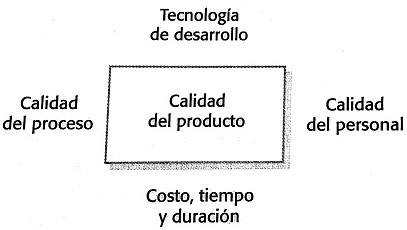
\includegraphics[scale=0.7]{M3-FactoresCalidad}
	\caption{Principales factores de calidad del producto de software \cite{sommerville_ingenierisoftware_2002}}\label{fig:M3-FactoresCalidad}
\end{figure}
\FloatBarrier

%Comentar fig 24.9 p549 relacion de metricas de proc y de prod

Para llegar a tener un software de calidad hay que tener en cuenta todos los factores mencionados anteriormente en cada una de las tres fases de la \textbf{administración de la calidad}: aseguramiento, planificación y control.

\begin{description}
	\item[Aseguramiento de la calidad.] Se encarga de establecer un marco de trabajo de procedimientos y estándares que guíen a construir software de calidad.
	\item[Planificación de la calidad.] Selección de procedimientos y estándares para un proyecto software específico.
	\item[Control de la calidad.] La fase de control es la que se encarga de que el equipo de desarrollo cumpla los estándares y procedimientos definidos en el plan de calidad del proyecto. Esta fase puede realizarse mediante revisiones de calidad llevados a cabo por un grupo de personas y/o mediante un proceso automático llevado a cabo por algún programa.
\end{description}

%Comentar fg 24.1 p537 admin de calida en el proceso y desarrollo de software

\subsection{Control de la calidad: medición}

En la fase de control de calidad se vigila que se sigan los procedimientos y estándares definidos en el plan de calidad. Pero estos podrían no ser adecuados o siempre pueden mejorar, por lo que en esta fase se puede valorar el mejorarlos como se puede observar en la Fig. \ref{fig:M3_CalidadProcesos}.

\imagen{M3_CalidadProcesos}{Calidad basada en procesos \cite{sommerville_ingenierisoftware_2002}}

Este proceso puede ser llevado a cabo mediante revisiones ejecutadas por un grupo de personas o por medio de programas que automaticen este proceso. El  desafío a la comunidad científica y empresarial es constante mostrando un incremento en el interés de aplicaciones que permiten  mejorar sus sistemas de decisión. Estas aplicaciones deberán llevar un control sobre el proceso y/o sobre el producto software y ese control se podrá realizar mediante un proceso de medición, que ofrece una medida cuantitativa de los atributos del producto y proceso software. 

La medición del software es un proceso en el que se asignan valores numéricos o simbólicos a atributos de un producto o proceso software. Una métrica de software es una medida cuantitativa del grado en que un sistema, componente o proceso software posee un atributo dado. Las métricas son de control o de predicción. Las \textbf{métricas de control} se asocian al proceso de desarrollo del software, por ejemplo, la media de días que se tarda en cerrar una incidencia; y las \textbf{métricas de predicción} se asocian a productos software, por ejemplo, la complejidad ciclomática de una función. Ambos tipos de métricas influyen en la toma de decisiones administrativas como se observa en la Fig. \ref{fig:M3-MetricasProcesoYProducto}. Los repositorios y las forjas facilitan la obtención de datos para este proceso de medición.

\imagen{M3-MetricasProcesoYProducto}{Métricas de control y métricas de predicción \cite{sommerville_ingenierisoftware_2002}}

Este proyecto se centra sólo en la obtención de métricas de evolución que permitirán controlar y evaluar el proceso del desarrollo de un producto software. Por tanto se dejarán las métricas de predicción para otros trabajos y se detallará más sobre las de control en el siguiente apartado.

\subsection{Métricas de control: medición de la evolución o proceso de software}\label{sect:3_3_2_MetricasControl}

En la Fig. \ref{fig:M3-FactoresCalidad} se muestra la calidad de proceso como factor que afecta directamente a la calidad de producto. Parece lógico considerar como hipótesis que la calidad de un artefacto software tenga alguna relación con la manera en la que el equipo de desarrollo aplica las actividades del ciclo de vida del software dentro del repositorio. La validación empírica de estas  hipótesis ha abierto una nueva línea de aplicación con los conjuntos de datos que se pueden extraer de los repositorios gracias a interfaces de programación específicas que proporcionan estas forjas de repositorios y que permiten acceder a toda la información registrada.

Una plataforma de desarrollo colaborativo como \textit{GitLab} puede presentar herramientas para controlar la evolución de un proyecto software, por ejemplo: un sistema de control de versiones (\textit{VCS} - \textit{Version Control System}), un sistema de seguimiento de incidencias (\textit{issue Tracking System}), un sistema de integración continua (\textit{CI} - \textit{Continuous Integration}), un sistema de despliegue continuo (\textit{CD} - \textit{Continuous Deployment}), etc.
Todas estas herramientas facilitan la comunicación entre los miembros de un equipo de desarrollo, ayudan a gestionar los cambios que producen cada uno de los miembros y proporcionan mediciones de proceso. Estas mediciones se pueden utilizar para obtener métricas de control que ayuden a evaluar y mejorar la evolución del proyecto.

Las métricas de control que se utilizan en este proyecto provienen de una \textit{Master Tesis} titulada \textit{sPACE: Software Project Assessment in the Course of Evolution} \cite{ratzinger_space:_2007}. 
A continuación se describen las métricas que se implementan en este proyecto usando la plantilla de definición de la norma ISO 9126.

Además, en esta segunda iteración del proyecto se han añadido cinco nuevas métricas relacionadas con la integración y despliegue continuo (\textit{CICD}).
 
\textbf{\underline{I1 - Número total de \textit{issues} (incidencias)}}

\begin{itemize}
	\item \textbf{Categoría}: Proceso de Orientación
	\item \textbf{Descripción}: Número total de \textit{issues} creadas en el repositorio
	\item \textbf{Propósito}: ¿Cuántas \textit{issues} se han definido en el repositorio?
	\item \textbf{Fórmula}: $NTI$. \textit{NTI = número total de \textit{issues}}
	\item \textbf{Fuente de medición}: Proyecto en una plataforma de desarrollo colaborativo.
	\item \textbf{Interpretación}: $NTI \geq 0$. Valores bajos indican que no se utiliza un sistema de seguimiento de incidencias, podría ser porque el proyecto acaba de comenzar
	\item \textbf{Tipo de escala}: Absoluta
	\item \textbf{Tipo de medida}: \textit{NTI = Contador}
\end{itemize}

\textbf{\underline{I2 - \textit{commits} (cambios) por \textit{issue}}}

\begin{itemize}
	\item \textbf{Categoría}: Proceso de Orientación
	\item \textbf{Descripción}: Número de \textit{commits} por \textit{issue}
	\item \textbf{Propósito}: ¿Cuál es el volumen medio de trabajo de las \textit{issues}?
	\item \textbf{Fórmula}: $CI = \frac{NTC}{NTI}$. \textit{CI = Cambios por \textit{issue}, NTC = Número total de \textit{commits}, NTI = Número total de \textit{issues}}
	\item \textbf{Fuente de medición}: Proyecto en una plataforma de desarrollo colaborativo.
	\item \textbf{Interpretación}: $CI \geq 1$, Lo normal son valores altos. Si el valor es menor que uno significa que hay desarrollo sin documentar.
	\item \textbf{Tipo de escala}: Ratio 
	\item \textbf{Tipo de medida}: \textit{NTC, NTI = Contador}
\end{itemize}

\textbf{\underline{I3 - Porcentaje de \textit{issues} cerradas}}

\begin{itemize}
	\item \textbf{Categoría}: Proceso de Orientación
	\item \textbf{Descripción}: Porcentaje de \textit{issues} cerradas
	\item \textbf{Propósito}: ¿Qué porcentaje de \textit{issues} definidas en el repositorio se han cerrado?
	\item \textbf{Fórmula}: $PIC = \frac{NTIC}{NTI}*100$. \textit{PIC = Porcentaje de \textit{issues} cerradas, NTIC = Número total de \textit{issues} cerradas, NTI = Número total de \textit{issues}}
	\item \textbf{Fuente de medición}: Proyecto en una plataforma de desarrollo colaborativo.
	\item \textbf{Interpretación}: $0 \leq PIC \leq 100$. Cuanto más alto mejor
	\item \textbf{Tipo de escala}: Ratio
	\item \textbf{Tipo de medida}: \textit{NTI, NTIC = Contador}
\end{itemize}

\textbf{\underline{TI1 - Media de días en cerrar una \textit{issue}}}

\begin{itemize}
	\item \textbf{Categoría}: Constantes de tiempo
	\item \textbf{Descripción}:  Media de días en cerrar una \textit{issue}
	\item \textbf{Propósito}: ¿Cuánto se suele tardar en cerrar una \textit{issue}? 
	\item \textbf{Fórmula}: $MDCI = \frac{\sum_{i=0}^{NTIC}DCI_i}{NTIC}$. \textit{MDCI = Media de días en cerrar una \textit{issue}, NTIC = Número total de \textit{issues} cerradas, DCI = Días en cerrar la \textit{issue}}
	\item \textbf{Fuente de medición}: Proyecto en una plataforma de desarrollo colaborativo.
	\item \textbf{Interpretación}: $MDCI \geq 0$. Cuanto más pequeño mejor. Si se siguen metodologías ágiles de desarrollo iterativo e incremental como SCRUM, la métrica debería indicar la duración del \textit{sprint} definido en la fase de planificación del proyecto. En SCRUM se recomiendan duraciones del \textit{sprint} de entre una y seis semanas, siendo recomendable que no exceda de un mes \cite{scrum_master_scrum_2019}.
	\item \textbf{Tipo de escala}: Ratio
	\item \textbf{Tipo de medida}: \textit{NTI, NTIC = Contador}
\end{itemize}

\textbf{\underline{TC1 - Media de días entre \textit{commits}}}

\begin{itemize}
	\item \textbf{Categoría}: Constantes de tiempo
	\item \textbf{Descripción}: Media de días que pasan entre dos \textit{commits} consecutivos
	\item \textbf{Propósito}: ¿Cuántos días suelen pasar desde un \textit{commit} hasta el siguiente?
	\item \textbf{Fórmula}: $MDC = \frac{\sum_{i=1}^{NTC} TC_i - TC_{i-1}}{NTC}$. $TC_i - TC_{i-1}$ en días; \textit{MDC = Media de días entre cambios, NTC = Número total de \textit{commits}, TC = Tiempo de \textit{commit}}
	%$MDEC = [Sumatorio de (TCi-TCj) desde i=1, j=0 hasta i=NTC] / NTC. NTC = Número total de \textit{commits}, TC = Tiempo de Commit$ 
	\item \textbf{Fuente de medición}: Proyecto en una plataforma de desarrollo colaborativo.
	\item \textbf{Interpretación}: $MDEC \geq 0$. Cuanto más pequeño mejor. Se recomienda no superar los 5 días.
	\item \textbf{Tipo de escala}: Ratio
	\item \textbf{Tipo de medida}: \textit{NTC = Contador; TC = Tiempo}
\end{itemize}

\textbf{\underline{TC2 - Días entre primer y último \textit{commit}}}

\begin{itemize}
	\item \textbf{Categoría}: Constantes de tiempo
	\item \textbf{Descripción}: Días transcurridos entre el primer y el último \textit{commit} 
	\item \textbf{Propósito}: ¿Cuantos días han pasado entre el primer y el último \textit{commit}?
	\item \textbf{Fórmula}: $DEPUC = TC2- TC1$. $TC2- TC1$ en días;  \textit{DEPUC = Días entre primer y último \textit{commit}, TC2 = Tiempo de último \textit{commit}, TC1 = Tiempo de primer \textit{commit}}
	\item \textbf{Fuente de medición}: Proyecto en una plataforma de desarrollo colaborativo.
	\item \textbf{Interpretación}: $DEPUC \geq 0$. Cuanto más alto, más tiempo lleva en desarrollo el proyecto. En procesos software empresariales se debería comparar con la estimación temporal de la fase de planificación. 
	\item \textbf{Tipo de escala}: Absoluta
	\item \textbf{Tipo de medida}: \textit{TC = Tiempo}
\end{itemize}

\textbf{\underline{TC3 - Ratio de actividad de \textit{commits} por mes}}

\begin{itemize}
	\item \textbf{Categoría}: Constantes de tiempo
	\item \textbf{Descripción}: Muestra el número de \textit{commits} relativos al número de meses
	\item \textbf{Propósito}:¿Cuál es el número medio de cambios por mes?
	\item \textbf{Fórmula}: $RCM = \frac{NTC}{NM}$. \textit{RCM = Ratio de cambios por mes, NTC = Número total de \textit{commits}, NM = Número de meses que han pasado durante el desarrollo de la aplicación}
	\item \textbf{Fuente de medición}: Proyecto en una plataforma de desarrollo colaborativo.
	\item \textbf{Interpretación}: $RCM > 0$. Cuanto más alto mejor
	\item \textbf{Tipo de escala}: Ratio
	\item \textbf{Tipo de medida}: \textit{NTC = Contador}
\end{itemize}

\textbf{\underline{C1 - Cambios pico}}

\begin{itemize}
	\item \textbf{Categoría}: Constantes de tiempo
	\item \textbf{Descripción}: Número de \textit{commits} en el mes que más \textit{commits} se han realizado en relación con el número total de \textit{commits}
	\item \textbf{Propósito}: ¿Cuál es la proporción de trabajo realizado en el mes con mayor número de cambios?
	\item \textbf{Fórmula}: $CP = \frac{NCMP}{NTC}$. \textit{CP = Cambios pico, NCMP = Número de \textit{commits} en el mes pico, NTC = Número total de \textit{commits}}
	\item \textbf{Fuente de medición}: Proyecto en una plataforma de desarrollo colaborativo.
	\item \textbf{Interpretación}: $0 \leq CCP \leq 1$. Mejor valores intermedios. Se recomienda no superar el 40\% del trabajo en un mes.
	\item \textbf{Tipo de escala}: Ratio
	\item \textbf{Tipo de medida}: \textit{NCMP, NTC = Contador}
\end{itemize}

\begin{large}
\textbf{\underline{Nuevas métricas relacionadas con \textit{CI-CD}}}
\linebreak
\end{large}

\textbf{\underline{IC1 - Número total de \textit{jobs} ejecutados}}
\begin{itemize}
	\item \textbf{Categoría}: CI-CD
	\item \textbf{Descripción}: Número de \textit{jobs} ejecutados en el proyecto.
	\item \textbf{Propósito}: ¿Cuál es el número total de de \textit{jobs} ejecutados con éxito en el proyecto?
	\item \textbf{Fórmula}: $NJE =$ \textit{número total de jobs}.
	\item \textbf{Fuente de medición}: Proyecto en una plataforma de desarrollo colaborativo.
	\item \textbf{Interpretación}: $NJE \geq 0$. Un valor de cero indica que el proyecto no tiene integración y despliegues continuos y no se ha realizado ningún trabajo automatizado de despliegue.
	\item \textbf{Tipo de escala}: Absoluta
	\item \textbf{Tipo de medida}: \textit{NJE = Contador}
\end{itemize}

\textbf{\underline{IC2 - Número de \textit{Jobs} ejecutados el último año}}
\begin{itemize}
	\item \textbf{Categoría}: CI-CD
	\item \textbf{Descripción}: Número de \textit{jobs} ejecutados en el último año (últimos 365 días).
	\item \textbf{Propósito}: ¿Cuál es el número total de \textit{jobs} ejecutados con éxito en el proyecto durante el año previo?
	\item \textbf{Fórmula}: $NJELY =$ \textit{número total de jobs ejecutados el útimo año}.
	\item \textbf{Fuente de medición}: Proyecto en una plataforma de desarrollo colaborativo.
	\item \textbf{Interpretación}: $NJELY \geq 0$. Un valor de cero indica que en el proyecto no se ha realizado ningún trabajo automatizado de despliegue durante el último año.
	\item \textbf{Tipo de escala}: Absoluta
	\item \textbf{Tipo de medida}: \textit{NJELY = Contador}
\end{itemize}

\textbf{\underline{IC3 - \textit Número de tipos diferentes de{jobs} ejecutados}}
\begin{itemize}
	\item \textbf{Categoría}: CI-CD
	\item \textbf{Descripción}: Número de tipos diferentes de \textit{jobs} ejecutados en el proyecto.
	\item \textbf{Propósito}: ¿Cuál es el número total de tipos de \textit{jobs} ejecutados con éxito en el proyecto?
	\item \textbf{Fórmula}: $NTJE =$ \textit{número total de tipos diferentes de jobs ejecutados en el proyecto}.
	\item \textbf{Fuente de medición}: Proyecto en una plataforma de desarrollo colaborativo.
	\item \textbf{Interpretación}: $NTJE \geq 0$. Un valor de cero indica que el proyecto no tiene integración y despliegues continuos y no se ha realizado ningún trabajo automatizado de despliegue.
	\item \textbf{Tipo de escala}: Absoluta
	\item \textbf{Tipo de medida}: \textit{NTJE = Contador}
\end{itemize}


\textbf{\underline{DC1 - \textit Número total de{releases}}}
\begin{itemize}
	\item \textbf{Categoría}: CI-CD
	\item \textbf{Descripción}: Número de \textit{releases} lanzadas en el proyecto.
	\item \textbf{Propósito}: ¿Cuál es el número total de \textit{releases} del  proyecto?
	\item \textbf{Fórmula}: $NRR =$ \textit{número total de releases lanzadas en el proyecto}.
	\item \textbf{Fuente de medición}: Proyecto en una plataforma de desarrollo colaborativo.
	\item \textbf{Interpretación}: $NRR \geq 0$. Un valor de cero indica que aún no se ha lanzado ninguna \textit{release} del proyecto.
	\item \textbf{Tipo de escala}: Absoluta
	\item \textbf{Tipo de medida}: \textit{NRR = Contador}
\end{itemize}

\textbf{\underline{DC2 - \textit Número de{releases} lanzadas el último año}}
\begin{itemize}
	\item \textbf{Categoría}: CI-CD
	\item \textbf{Descripción}: Número de \textit{releases} lanzadas en el proyecto en el último año (últimos 365 días).
	\item \textbf{Propósito}: ¿Cuál es el número total de \textit{releases} lanzadas en el proyecto durante el año previo?
	\item \textbf{Fórmula}: $NRRLY =$ \textit{número total de releases lanzadas en el proyecto en el último año}.
	\item \textbf{Fuente de medición}: Proyecto en una plataforma de desarrollo colaborativo.
	\item \textbf{Interpretación}: $NRRLY \geq 0$. Un valor de cero indica que no se ha lanzado ninguna \textit{release} del proyecto durante el último año.
	\item \textbf{Tipo de escala}: Absoluta
	\item \textbf{Tipo de medida}: \textit{NRRLY = Contador}
\end{itemize}



\subsection{\textit{Framework} de medición}\label{sect:3_3_3_FrameworkMedicion}

Para la implementación de las métricas se ha seguido la solución basada en \textit{frameworks} propuesta en \textit{Soporte de Métricas con Independencia del Lenguaje para la Inferencia de Refactorizaciones} \cite{marticorena_sanchez_soporte_2005}. El objetivo del \textit{framework} es la reutilización en la implementación del cálculo de métricas. El diseño, mostrado en la Fig. \ref{fig:MCTMotorMetricas}, permite:

\begin{itemize}
	\tightlist
	\item Facilitar el desarrollo de nuevas métricas
	\item Personalizar los valores límite inferior y superior, puesto que éstos pueden variar dependiendo del contexto en el que se calculen las métricas.
	\item Crear un grupo de configuraciones de métricas llamado `Perfil de métricas' para poder evaluar los proyectos en torno a un contexto. Dos casos de ejemplo serían:
	\begin{itemize}
		\tightlist
		\item Crear un perfil de métricas para un grupo de trabajo que se encargue de software de finanzas y evaluar un proyecto respecto de proyectos ya terminados o respecto de proyectos públicos.
		\item Crear un perfil que evalúe las métricas de proyectos de fin de grado.
	\end{itemize}
\end{itemize}

\imagen{MCTMotorMetricas}{Diagrama del \textit{framework} para el cálculo de métricas con perfiles que almacena valores umbrales.}

En el diagrama UML de la Fig. \ref{fig:MCTMotorMetricas} se muestran las entidades principales del \textit{framework} de medición y la relación entre ellas, especificando la navegabilidad y la multiplicidad. Las anotaciones en forma de flecha oscura especifican los patrones de diseño \cite{gamma_patrones_2002} aplicados en el \textit{framework}.

Para crear una nueva métrica, esta deberá implementar la clase abstracta \textit{Metric}, en especial los métodos \textit{check()} y \textit{run()}. El método \textit{calculate()} de la clase \textit{Metric} utiliza el patrón de diseño \textbf{método plantilla}\footnote{\url{https://refactoring.guru/design-patterns/template-method}} sobre estos métodos, que deberán ser implementados por las clases concretas que hereden de \textit{Metric}. Un ejemplo de este método sería:

\begin{minipage}{\linewidth}
%{\tiny
\begin{verbatim}
...
Value calculate(Entity entity, 
		MetricConfiguration metricConfig, 
		MetricsResults metricsResults) 
{
  Value value;
  if(check(entity))
  {
    value = run(entity);
    metricsResults.addMeasure(new Measure(metricConfig, value));
  }
  return value;
}
...
\end{verbatim}
%}
\end{minipage}

Siendo \textit{entity} la entidad que se está midiendo, \textit{metricConfig} la configuración de valores límite que se está utilizando, \textit{metricsResults} el lugar donde se almacena el resultado y \textit{value} el valor medido en el método \textit{run()}. La plantilla establece una comprobación previa de que el repositorio contenga datos esenciales para el cálculo de la métrica, en ese caso se calcula la métrica y se añade el resultado a la coleción \textit{metricsResults}. 
Este método delega en las subclases el comportamiento de los métodos \textit{check} y \textit{run}. Además, almacena en el objeto colector \textit{metricsResults}, pasado como argumento, el valor medido para la configuración de la métrica para posibilitar el análisis y presentación de los resultados posteriores.

\textit{MetricConfiguration} toma el rol de decorador en el patrón de diseño \textbf{decorador}\footnote{\url{https://refactoring.guru/design-patterns/decorator}} que permite configurar los valores límite de las métricas. Implementa la misma interfaz que \textit{Metric}, \textit{IMetric}, y está asociado a una métrica. Su método \textit{calculate} simplemente realizará una llamada al método \textit{calculate} de la métrica (\textit{Metric}) a la que está asociada la configuración.

Un perfil de métricas agrupa un conjunto de configuraciones de métricas para un contexto dado, por ejemplo, para un conjunto de proyectos realizados por alumnos de la universidad en su realización del TFG. Se podría instanciar un \textit{MetricResult} para almacenar los resultados de toda esta colección de configuraciones de métricas y bastaría sólo con recorrer el perfil usando el método \textit{calculate()} de cada configuración.

Este TFG ha adaptado este \textit{framework} en el paquete ``motor de métricas'', y se han realizado unas pocas modificaciones. Las modificaciones más destacadas son:

\begin{itemize}
	\tightlist
	\item Se ha aplicado a las métricas concretas el patrón \textit{\textbf{Singleton}} \footnote{\url{https://refactoring.guru/design-patterns/singleton}}, que obliga a que sólo haya una única instancia de cada métrica; y se ha aplicado el patrón \textit{\textbf{Método fábrica}} \footnote{\url{https://refactoring.guru/design-patterns/factory-method}} tal y como se muestra en la Fig. \ref{fig:M3_CambiosFrameworkMedicion1}, de forma que \textit{MetricConfiguration} no esté asociada con la métrica en sí, sino con una forma de obtenerla.\\
	La intencionalidad de esto es facilitar la persistencia de un perfil de métricas. Las métricas se podrían ver como clases estáticas, no varían en tiempo de ejecución y solo debería haber una instancia de cada una de ellas. Por ello, al importar o exportar un perfil de métricas con su conjunto de configuraciones de métricas, estas configuraciones no deberían asociarse a la métrica, sino a la forma de acceder a la única instancia de esa métrica. 
	\item Se han añadido los métodos \textit{evaluate} y \textit{getEvaluationFunction} en la interfaz \textit{IMetric}, ver Fig. \ref{fig:M3_CambiosFrameworkMedicion2}.\\
	Esto permitirá interpretar y evaluar los valores medidos sobre los valores límite de la métrica o configuración de métrica. Por ejemplo, puede que para unas métricas un valor aceptable esté comprendido entre el valor límite superior y el valor límite inferior; y para otras un valor aceptable es aquel que supere el límite inferior.\\
	\textit{EvaluationFunction} es una interfaz funcional \footnote{Enlaces a la documentación: \url{https://docs.oracle.com/javase/8/docs/api/java/lang/FunctionalInterface.html} --- \url{https://docs.oracle.com/javase/8/docs/api/java/util/function/package-summary.html}} 
	de tipo `\textit{función}': recibe uno o más parámetros y devuelve un resultado. Este tipo de interfaces son posibles a partir de la versión 1.8 de Java.\\
	Esto permite definir los tipos de los parámetros y de retorno de una función que se puede almacenar en una variable. De este modo se puede almacenar en una variable la forma en la que se puede evaluar la métrica.
\end{itemize}

\imagen{M3_CambiosFrameworkMedicion1}{Patrones ``singleton'' y ``método fábrica'' sobre el \textit{framework} de medición}

\imagen{M3_CambiosFrameworkMedicion2}{Añadido al \textit{framework} de medición la evaluación de métricas}
\capitulo{4}{Técnicas y herramientas}

%Esta parte de la memoria tiene como objetivo presentar las técnicas metodológicas y las herramientas de desarrollo que se han utilizado para llevar a cabo el proyecto. Si se han estudiado diferentes alternativas de metodologías, herramientas, bibliotecas se puede hacer un resumen de los aspectos más destacados de cada alternativa, incluyendo comparativas entre las distintas opciones y una justificación de las elecciones realizadas. 
%No se pretende que este apartado se convierta en un capítulo de un libro dedicado a cada una de las alternativas, sino comentar los aspectos más destacados de cada opción, con un repaso somero a los fundamentos esenciales y referencias bibliográficas para que el lector pueda ampliar su conocimiento sobre el tema.
A continuación se muestran las diferentes técnicas y herramientas empleadas en el proyecto.

\section{Herramientas utilizadas}

En está sección se describen brevemente las herramientas utilizadas en el desarrollo del proyecto. La elección de las herramientas condicionada por el desarrollo previo, ha sido actualizada con versiones más recientes. En esta sección también se describen las notas de las acciones llevadas a cabo en durante el proceso de actualización. 
Se podrá encontrar más información acerca del código y las herramientas utilizadas en el 
`Apéndice D - Documentación técnica de programación'.


\subsection{Entorno de desarrollo}\label{sect:4_1_1_HerramientasDesarrollo}
%\todo En todas las herramientas describir brevemente las funcionalidades de que se utilizan concretamente en el proyecto.
%\todo Se pueden acompañar con alguna captura de pantalla, porción de código y a una referencia al manual del progromador para obtener más detalle.
%\todo Por ejemplo Java SE v11.0.1 Expresiones Lambda en el uso de stream. 
% \todo Apache Maven indicar brevemente el  flujo de trabajo utilizado de compilación, testing, calidad, package y despliegue 
El entorno de desarrollo lo componen las diferentes herramientas que se utilizan para realizar y facilitar el desarrollo del software,

\begin{description}
	\item[Eclipse IDE for Java EE Developers.] Entorno de programación Java para aplicaciones Web. 
	
		Se ha utilizado la versión: 2019-03. Enlace a página de descarga:
		
		\url{https://www.eclipse.org/downloads/packages/release/2019-03}
	
		Eclipse es uno de los IDE (Integrated Development Environment o entorno de desarrollo integrado por sus siglas en inglés) más empleados para el desarrollo en Java, aunque hay otros también muy utilizados como Intellij IDEA de JetBrains.
		
		\textit{Eclipse IDE for Java EE Developers} es un paquete que incluye herramientas para desarrolladores de Java que crean Java EE y aplicaciones web, incluido un IDE de Java, herramientas para Java EE, JPA, JSF, Mylyn, EGit y otros.
		
Más concretamente, el paquete incluye:
\begin{itemize}
\item Data Tools Platform
\item Eclipse Git Team Provider
\item Eclipse Java Development Tools
\item Eclipse Java EE Developer Tools
\item JavaScript Development Tools
\item Maven Integration for Eclipse
\item Mylyn Task List
\item Eclipse Plug-in Development Environment
\item Remote System Explorer
\item Eclipse XML Editors and Tools
\end{itemize}

Podemos obtener la versión más reciente en: \url{https://www.eclipse.org/downloads/packages/release/kepler/sr2/eclipse-ide-java-ee-developers}
		
		De forma adicional a las herramientas anteriores, es posible instalar \textbf{plugins} para ampliar la funcionalidad. En el proyecto se han instalado los siguientes:
	\begin{itemize}
		\item \textit{YEdit} para facilitar el trabajo con ficheros con un formato especial
		\item \textit{YEdit} sirve como editor de ficheros con extensión \textit{.yml}, y ha sido utilizado para generar los archivos que se usan para configurar la integración y despliegue continuo (tanto en Gitlab como GitHub).
		\item \textit{Vaadin Plugin for Eclipse 4.0.2}, sirve para poder usar la herramienta Vaadin en el entorno de Eclipse de una manera más sencilla.
	\end{itemize}
		
		Eclipse dispone de varias vistas para las diferentes tareas del proyecto, las más utilizadas han sido:
		\begin{itemize}
			\item \textbf{Java EE}. Es la vista por defecto de este paquete de Eclipse. Facilita el trabajo de aplicaciones Web y es la vista utilizada para escribir código. Ofrece, entre otras cosas, un explorador de paquetes y vistas para trabajar con Java.
			\item \textbf{Debug}. La vista utilizada para depurar el programa. Sirve para ejecutar la aplicación instrucción a instrucción y detectar así un problema o \textit{bug}.
			\item \textbf{Git}. Esta vista permite trabajar con el sistema de control de versiones Git. Mantiene una vista con un listado de repositorios, otra que visualiza el historial de cambios de un archivo seleccionado y, la más importante, una ventana que permite visualizar los cambios realizados, indexarlos, realizar commits y publicarlos en el repositorio remoto. Eclipse permite la integración con GitLab y cualquier otra forja de repositorios como GitHub.
			De forma adicional se ha trabajado con la consola de Git para Windows \textit{GitBash}.
		\end{itemize}
		
	\item[Java SE 11 (JDK).] \textit{Java Development Kit}. Conjunto de herramientas software útiles para el desarrollo de aplicaciones en Java entre las que se incluyen \textit{javac.exe}, el compilador de Java; \textit{javadoc.exe}, el generador de documentación; y \textit{java.exe}, el intérprete de Java.
	
		Se ha utilizado la versión  v11.0.1. Enlace a página de descarga:
		
		\url{https://www.oracle.com/java/technologies/downloads/}
	
		A pesar de haber utilizado la versión \textit{Java SE 11.0.2} \footnote{Actualmente ha sido lanzada la versión \textit{Java SE 17.0.2} y se esperan actualizaciones cada 6 meses.} de Java. Sin embargo, ha sido posible compilar y ejecutar tanto las pruebas como la aplicación Web con Java 8 realizando dos pequeñas modificaciones:
		\begin{itemize}
			\item De la versión 11 se ha utilizado el método \textit{isBlank()} de la clase \textit{String}. Se diferencia de \textit{isEmpty()} en que no comprueba la longitud de la cadena y devuelve \textit{true} si es 0, sino que devuelve \textit{true} si la longitud es 0 o si no es 0 pero todos los caracteres de la cadena son espacios en blanco.
			\item De la clase \textit{java.util.Optional} \footnote{\url{https://docs.oracle.com/en/java/javase/11/docs/api/java.base/java/util/Optional.html}}, soportada desde la versión 1.8, se utiliza la función \textit{orElseThrow()}, que se soporta desde la versión 10, por tanto habría que buscar una alternativa para pasar a la versión 1.8. La versión 11 trae a esta clase la función \textit{isEmpty()}.
		\end{itemize}
	\item[Apache Maven.] Gestor de proyectos software que ayuda en la construcción del proyecto, la generación de documentación, generación de informes, gestión de dependencias, integración continua dentro de forjas de repositorios como Github y GitLab, etc. 
	
		Se ha actualizado a la versión v3.8.0 desde la versión  v3.8.4 que utilizaba el proyecto original \cite{TFGPrevio}. Enlace a página de descarga:
		
		\url{https://maven.apache.org/download.cgi}
		
		Se han automatizado en este proyecto utilizando Maven y la integración continua de GitHub (\textit{Github Actions}) los siguientes procesos:
		\begin{itemize}
			\item Compilación. Es un proceso de generación de binarios a partir del código fuente escrito en Java.
			\item Pruebas unitarias y de integración automáticas con JUnit.
			\item Generación de informes de pruebas, cobertura y análisis de calidad con ayuda de Jacoco, JUnit y Codacy.
			\item Despliegue en servidor de Heroku.
		\end{itemize}
	
	\item[Maven Jetty Plugin.] Contenedor de aplicaciones Web integrado con Maven en forma de plugin.
	
		Se ha utilizado la versión  v9.4.36 y se ha incluido en el proyecto en el pom.xml:
	
\begin{verbatim}
...
<plugin>
	<groupId>org.eclipse.jetty</groupId>
	<artifactId>jetty-maven-plugin</artifactId>
	<version>9.4.36.v20210114</version>
	<configuration>
		<scanIntervalSeconds>2</scanIntervalSeconds>
	</configuration>
</plugin>
...
\end{verbatim}
		
Enlace a página de descarga:
		
		\url{https://mvnrepository.com/artifact/org.eclipse.jetty/jetty-maven-plugin/9.4.36.v20210114}
		
Se ha utilizado para desplegar en el equipo local de desarrollo y realizar pruebas durante el desarrollo en local. Para correr la aplicación en el entorno local basta con ejecutar: 
		
\begin{verbatim}
mvn jetty:run
\end{verbatim}

y gracias a la capacidad que tiene el plugin de captar los cambios (cada dos segundos según podemos ver en la configuración previa) facilita mucho el desarrollo al recompilar automáticamente el proyecto.
		
\end{description}
\subsection{Logging}
El \textit{logging} es el proceso que permite ver lo que ocurre durante la ejecución de la aplicación para poder depurar errores y analizar comportamientos para solucionar diferentes problemas. Este proceso es útil tanto en la fase de desarrollo del proyecto como en la de producción una vez la aplicación está desplegada y en uso por usuarios finales.

\begin{description}
	\item[SLF4J.] Visualización del \textit{logging}.
	Sirve como una simple fachada o abstracción para varios marcos de registro (por ejemplo, java.util.logging, logback, log4j) que permite al usuario final conectar el marco de registro deseado en el momento de la implementación.
	
		Enlace a página de descarga:
	
		\url{https://www.slf4j.org/download.html}
	
	\item[Log4j 2.] Logger. Se ha utilizado actualizado la versión a la 2.17.2 desde v2.11.2 utilizada por el proyecto previo \cite{TFGPrevio} para evitar diferentes vulnerabilidades.
	
	 	Enlace a página de descarga:
	
	 	\url{https://mvnrepository.com/artifact/org.apache.logging.log4j/log4j-core/2.17.2}\\
		
		Esta herramienta permite configurar este proceso por medio de un fichero log4j2 con extensión XML, JSON, YAML o Properties\footnote{Manual de configuración de Log4j 2: \url{https://logging.apache.org/log4j/2.x/manual/configuration.html}} \cite{apache_apache_nodate}. En este proyecto se configuró mediante un fichero con extensión \textit{.properties}. 
		
		Ambas herramientas están integradas con Maven, y solo es necesario añadir en el fichero \ruta{pom.xml} las dependencias correspondientes.
	
\end{description}
\subsection{Pruebas}
La fase de pruebas permite comprobar que la implementación realizada funciona correctamente y no contiene errores. Se han implementado dos tipos de pruebas: unitarias y de integración. Las unitarias prueban los diferentes módulos y las de integración prueban la relación que tienen los diferentes módulos entre sí.
\begin{description}
	\item[JUnit5]. Conjunto de bibliotecas para el desarrollo de pruebas unitarias. 
	
		Se ha utilizado la versión  v5.3.1. Enlace a página de descarga:
		
		\url{https://junit.org/junit5/}
		
		JUnit permite realizar pruebas unitarias de forma automática o semiautomática de aplicaciones Java. Se han ejecutado de ambas formas en el proyecto. La automatización completa ha sido posible gracias a las herramientas de CI (\textit{Continuous Integration}) de Github \textit{GitHub Actions}: 
		\url{https://docs.github.com/es/actions}
		
		Esta versión de JUnit 5, sobre la anterior JUnit 4, ha influido en este proyecto de la siguiente manera:
		\begin{itemize}
			\item JUnit 5 soporta \textbf{Java 11}.
			
			\item Permite realizar asertos (\textit{asserts}) de tipo \textit{\textbf{assertAll()}} \footnote{\url{https://junit.org/junit5/docs/current/api/org/junit/jupiter/api/Assertions.html}}. Este tipo de asertos permite tratar varios asertos como una unidad. Se utilizaron en versiones anteriores de la aplicación, pero realmente no eran necesarios y se optó por quitarlos.
			
			\item Permite realizar \textbf{comprobaciones de lanzamiento de excepciones} en asertos del tipo \textit{assertThrows()}.
			
			\item Permite realizar suposiciones (\textit{\textbf{assumptions}}) que permiten realizar una comprobación que pasará por alto un test (lo marca como \textit{skipped}) si la comprobación falla. Es decir que no lo marcará como error, simplemente no realizará el test. 
			\\Esto ha sido útil de cara a probar funciones que realizan conexiones a GitLab o GitHub que requieren credenciales de acceso que no se pueden publicar en los test ya que quedarían publicadas. Por tanto estos test tienen presunciones que comprueban que se tiene las credenciales de acceso y no se realizan los test si no se dispone de estas credenciales, en lugar de lanzar un error por no poder realizar la conexión.
			\\Estos test se ejecutan manualmente por el programador en su equipo local y no se ejecutan automáticamente en el proceso de integración continua.
			
			\item Permite crear \textbf{test parametrizados}. Estos son test que prueban funciones que requieren argumentos. Cada combinación de argumentos es un caso de prueba, y crear un test para cada combinación es un caso claro del defecto de código: `código duplicado'. Por ello estos argumentos se pueden generar mediante funciones, enumeraciones, proveedores de argumentos o recolectar desde un CSV y solo ser necesario un test para todas las combinaciones de argumentos posibles.
		\end{itemize}
\end{description}
\subsection{Frameworks y librerías específicas para el proyecto}
\begin{description}
	\item[github-api.kohsuke]. Librería de conexión a GitHub API. 
	
		Se ha utilizado esta librería para realizar la conexión con la API de Github en su última versión disponible, la 1.306:
		
		\url{https://github-api.kohsuke.org/}
		
		
	\item[gitlab4j-api]. Framework de conexión a GitLab API. 
	
		Se ha actualizado a última versión disponible, la versión  v4.19.0. Enlace:
		
	\url{https://javadoc.io/doc/org.gitlab4j/gitlab4j-api/4.19.0/index.html}
		
		
			
	\item[Apache Commons Math]. Librería que se utiliza para matemáticas descriptivas y que ha servido para el cálculo de cuartiles, necesarios para obtener los valores umbrales de las métricas según las estadísticas. 
	
		Se ha utilizado la versión  v3.6.1. Enlace a página de descarga:
	
		\url{https://commons.apache.org/proper/commons-math/download_math.cgi}
		
		Ejemplo de uso de la clase \textit{DescriptiveStatistics} de la librería:
		
\begin{minipage}{\linewidth}
{\tiny 
\begin{verbatim}[breaklines]
...
ArrayList<Double> datasetForMetric;
Double q1ForMetric, q3ForMetric;
DescriptiveStatistics descriptiveStatisticsForMetric;

descriptiveStatisticsForMetric = new DescriptiveStatistics(datasetForMetric
	  .stream()
	  .mapToDouble(x -> x)
	  .toArray());
q1ForMetric = descriptiveStatisticsForMetric.getPercentile(25);
q3ForMetric = descriptiveStatisticsForMetric.getPercentile(75);
...
\end{verbatim}
}
\end{minipage}		

\end{description}
\subsection{Interfaz gráfica}
\begin{description}
	\item[Vaadin]. Framework para desarrollo de interfaces Web con Java.
		Se ha utilizado la versión  v13.0.0 Enlace:
		
		\url{https://vaadin.com/}
		
		Con este framework no ha sido necesario escribir HTML, solo Java y CSS para los estilos. 
		\\Como ejemplo de esto, para implementar un \textit{input} se utilizaría el siguiente código:
		
\begin{minipage}{\linewidth}
\tiny \begin{verbatim}
...
EmailField emailField = new EmailField();
emailField.setLabel("Email address");
add(emailField);
...
\end{verbatim}
\end{minipage}	

		y el resultado sería el de las siguientes figuras Fig. \ref{fig:M4_Vaadin_Input_1} y Fig. \ref{fig:M4_Vaadin_Input_2}
\begin{figure}[!h]
	\centering
	
\includegraphics[scale=0.5]{M4_Vaadin_Input_1}
	\caption{Input generado por Vaadin vacío}\label{fig:M4_Vaadin_Input_1}
	
	
	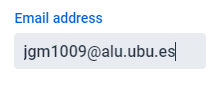
\includegraphics[scale=0.5]{M4_Vaadin_Input_2}
	\caption{Input generado por Vaadin con texto}\label{fig:M4_Vaadin_Input_2}
\end{figure}
\FloatBarrier

\end{description}
\subsection{Desarrollo y despliegue continuo}
\begin{description}
	\item[GitHub]. Forja (plataforma de desarrollo colaborativo) para alojar proyectos utilizando el sistema de control de versiones Git en la que se ha almacenado el proyecto en un repositorio Git.
	
		Enlace a GitHub:
		
		\url{https://github.com/}
		
		Enlace al repositorio del proyecto:
		
		\url{https://github.com/Joaquin-GM/GII_O_MA_19.07-Comparador-de-metricas-de-evolucion-en-repositorios-Software}
		
		En este proyecto se ha optado por utilizar GitHub frente a la primera iteración del proyecto \cite{TFGPrevio} para explorar su funcionalidad y comprobar que también es utilizable. Para más información hay una comparativa entre GitHub y GitLab en la sección \ref{sect:3_2_1_GitHubVSGitLab}.
		
	\item[Codacy]. Herramienta de generación automática de informes de calidad de código.
	
		 Enlace a Codacy:
		 
		 \url{https://www.codacy.com/}
		 
		 Enlace a proyecto en Codacy: 
		 
		 % TODO -> cuando esté generado poner el enlace al manual del proyecto
		 \url{https://app.codacy.com}
	
	\item[JaCoCo]. Librería utilizada para generar informes de cobertura del código en Java. Estos informes se pueden mostrar en GitHub fácilmente publicando los informes con formato HTML. También se han enviado estos informes a Codacy para que controle la cobertura además de la calidad de código.
	
		Se ha actualizado al proyecto para usar la la versión v0.8.7. 
		
		Enlace:
		
		\url{https://www.eclemma.org/jacoco/}
		
		Enlace a informe de JaCoCo en HTML sobre la cobertura del proyecto:
		
		% TODO -> cuando esté generado el primer nuevo informe poner url
		% \url{}
	
	\item[Heroku]. Herramienta para despliegue continuo (CD).
	
		Enlace a herramienta:
		
		\url{https://id.heroku.com/login}
		
		Enlace a aplicación desplegada:
		
		\url{https://evolution-metrics-v2.herokuapp.com/}
	
\end{description}
\subsection{Documentación}
\begin{description}
	\item[LaTeX]. Sistema de composición de textos.
		Enlace a herramienta:
		
		\url{https://www.latex-project.org/}
		
	\item[TeXMaker]. Entorno de desarrollo de documentos LaTeX.
	
		Enlace a herramienta:
		
		\url{https://www.xm1math.net/texmaker/}
	
	\item[Zotero]. Herramienta de gestión de fuentes bibliográficas.
		
		Enlace a herramienta:
		
		\url{https://www.zotero.org/}
	
\end{description}
\section{Técnicas}
\begin{itemize}
	\item A lo largo del proyecto se han utilizado diferentes patrones de diseño \cite{gamma_patrones_2002} como Singleton, Factory Method, Wrapper, Builder, Listener, etc.En los apéndices se puede encontrar más información al respecto.
	
	\item Para el motor de métricas se ha utilizado como base el framework propuesto en \textit{Soporte de Métricas con Independencia del Lenguaje para la Inferencia de Refactorizaciones} \cite{marticorena_sanchez_soporte_2005}. Ver Fig. \ref{fig:MCTMotorMetricas} en la sección \ref{sect:3_3_3_FrameworkMedicion}.
	
	\item El ciclo de vida del software de este proyecto se ha basado en \textit{Scrum}\cite{scrum_master_scrum_2019}, es decir, ha seguido un modelo de proceso iterativo e incremental. En el documento de anexos en su primera sección titulada Plan de proyecto se mostrarán los detalles de las iteraciones.
\end{itemize}

\capitulo{5}{Aspectos relevantes del desarrollo del proyecto}

%Este apartado pretende recoger los aspectos más interesantes del desarrollo del proyecto, comentados por los autores del mismo.
%Debe incluir desde la exposición del ciclo de vida utilizado, hasta los detalles de mayor relevancia de las fases de análisis, diseño e implementación.
%Se busca que no sea una mera operación de copiar y pegar diagramas y extractos del código fuente, sino que realmente se justifiquen los caminos de solución que se han tomado, especialmente aquellos que no sean triviales.
%Puede ser el lugar más adecuado para documentar los aspectos más interesantes del diseño y de la implementación, con un mayor hincapié en aspectos tales como el tipo de arquitectura elegido, los índices de las tablas de la base de datos, normalización y desnormalización, distribución en ficheros3, reglas de negocio dentro de las bases de datos (EDVHV GH GDWRV DFWLYDV), aspectos de desarrollo relacionados con el WWW...
%Este apartado, debe convertirse en el resumen de la experiencia práctica del proyecto, y por sí mismo justifica que la memoria se convierta en un documento útil, fuente de referencia para los autores, los tutores y futuros alumnos.

%Despliegue continuo - direccion de app en heroku. Sistema gratuito sirve para validar, pero no para explotar
%Diseño extensible
%Framework vaadin
%No responsive

En este capítulo se recogen los aspectos más interesantes del desarrollo del proyecto y se justifican las diferentes decisiones tomadas durante el mismo. Se hace mención al motivo de elección del proyecto, el modelo del ciclo de vida empleado, el flujo de trabajo y la configuración del proyecto.


\section{Selección del proyecto}

La elección de este proyecto se debe a su temática de análisis de repositorios. Trata un aspecto al que normalmente no se presta demasiada atención en el desarrollo de proyectos software. Según la experiencia laboral del alumno, normalmente se presta más atención a métricas de proyecto y se descuidan las del proceso, olvidando cuidar la administración de la calidad correctamente.
Esto es un error ya que analizando los repositorios con los que trabajamos en el desarrollo de proyectos podemos obtener métricas que nos dan información muy valiosa. Con esta información podemos detectar problemas que antes pasaban desapercibidos y mejorar en mucho la productividad de los equipos modificando ciertos aspectos del proceso de desarrollo.
En este proyecto se han utilizado métricas que permiten llevar un control sobre el ciclo de vida de uno o varios proyecto, haciendo posible comparar su evolución a lo largo del tiempo. Además, permiten comparar si se están cumpliendo los objetivos definidos y como se mencionaba anteriormente mejorar el proceso de desarrollo aumentando su calidad.

En cuanto a la relación del proyecto con las diferentes asignaturas del Grado, está principalmente relacionado con la asignatura \textit{Desarrollo Avanzado de Sistemas Software}, donde se trata como desarrollar software de calidad mediante el proceso de \textit{Administración de la calidad}, en el cual una de las actividades es el control de calidad. Este control se puede llevar a cabo mediante un proceso de medición utilizando diferentes métricas.


Otras asignaturas relacionadas: 
\begin{itemize}
	\tightlist
	\item \textit{Metodología de la Programación} y \textit{Estructuras de Datos} han contribuido en cuanto a la construcción de una aplicación en un lenguaje Orientado a Objetos.	
		\item \textit{Ingeniería del Software}: ciclo de vida del software, el análisis de los requisitos y el modelado del sistema (diagramas de clases, diagramas de casos de uso, etc).
		\item \textit{Análisis y Diseño de Sistemas}: comprensión del sistema desarrollado en la aplicación Web ya existente \cite{TFGPrevio} de forma que se puedan realizar nuevas implementaciones y mejoras.
	\item \textit{Estadística}: comprensión del cálculo de cuartiles para calcular los valores umbrales de las métricas.
	\item \textit{Interacción Hombre/Máquina}: comprensión de los aspectos fundamentales para mejorar la usabilidad, simplicidad, adaptabilidad de la interfaz gráfica.
	\item \textit{Diseño y Mantenimiento del Software}, el uso de patrones de diseño para mejorar la calidad de código y mantener los principios SOLID  \footnote{Single responsability, Open/Closed, Liskov substitution, Interface segregation, Dependency inversion} y de \textit{Desarrollo Avanzado de Sistemas Software} la naturaleza del trabajo, las revisiones automáticas de calidad de código por medio de métricas y la importancia de la refactorización al detectar defectos de diseño.
	\item \textit{Validación y Pruebas} comprensión de las pruebas ya desarrolladas y construcción de nuevas.
	\item \textit{Sistemas Distribuidos} ha ayudado en el uso de Maven y en la construcción de una aplicación Web.
	\item \textit{Gestión de Proyectos}: ciclo de vida de desarrollo empleado durante el proyecto: \textit{Scrum}\cite{scrum_master_scrum_2019}.
\end{itemize}

\newpage

\section{Modelo de ciclo de vida}
La metodología utilizada durante el desarrollo del proyecto ha sido \textit{\textbf{Scrum}}, realizándose un proceso incremental, dividido en \textit{sprints} de dos semanas. A la finalización de cada \textit{sprint} se ha realizado una reunión denominada \textit{sprint review} que que se compone de dos partes:
\begin{description}
	\item [Revisión del sprint:] o \textit{sprint review}, donde se comentan los avances realizados así como los diferentes problemas que han surgido durante las dos semanas de duración del \textit{sprint}.
Se modifica la pila de desarrollo (\textit{sprint backlog}) pasando a completadas aquellas historias de usuario finalizadas y al siguiente \textit{sprint} las no finalizadas, comentando posibles mejoras y soluciones a los problemas que se hayan tenido \cite{scrum_master_scrum_2019}.

	\item [Planificación del siguiente sprint:] o \textit{sprint planning}, donde e definen las tareasa abordar  durante el siguiente sprint. Estas tareas se recogen del \textit{product backlog} o pila de producto y se añaden a la pila del sprint o \textit{sprint backlog}.
\end{description}

	Concretamente, se ha utilizado \textbf{ZenHub} en conjunto a las \textit{issues} de GitHub para la gestión del proceso \textit{Scrum} en el proyecto.

A lo largo del desarrollo del proyecto, los \textit{sprints} se han centrado en diferentes tareas como pueden ser:
\begin{itemize}
	\item  Tareas de \textbf{investigación}, tanto de las materias relacionadas con el proyecto como de las herramientas que se utilizarán durante el proceso y de \textbf{configuración} del entorno de desarrollo.
	\item En la segunda etapa se aprecian tareas de \textbf{diseño e implementación} de la parte lógica de la aplicación. Se diseña el framework de conexión a forjas de repositorios, se implementa el framework descrito en \textit{Soporte de Métricas con Independencia del Lenguaje para la Inferencia de Refactorizaciones}  \cite{marticorena_sanchez_soporte_2005} para el cálculo de métricas y se diseñan los modelos de datos que serán utilizados por la aplicación.
	\item Tareas de \textbf{desarrollo} de las nuevas funcionalidades del proyecto, como la integración con GitHub, utilizando como base el framework descrito en \textit{Soporte de Métricas con Independencia del Lenguaje para la Inferencia de Refactorizaciones}  \cite{marticorena_sanchez_soporte_2005} y la integración ya existente con GitLab. Nuevos tests y mejoras de diferentes interfaces.
	\item Tareas de \textbf{integración y despliegue continuo} (CI/CD), configurando GitHub Actions y el resto de herramientas para el flujo de trabajo de los sprints.
	\item Revisión de las \textbf{pruebas unitarias} existentes y creación de nuevas con JUnit. automatizando su ejecución gracias a Maven y los \textit{pipelines} \footnote{Definen las actividades de los procesos de CI/CD y las fases y el entorno en las que se ejecutarán} de GitHub Actions.
		\item Configurar \textbf{revisiones automáticas de calidad} y de cobertura de las pruebas gracias a Maven, Codacy, JaCoCo y GitHub.
	\item Configuración y puesta a punto de un entorno en Heroku donde realizar el \textbf{despliegue} la aplicación durante las tareas de de CI/CD.
	\item Revisión y configuración de \textbf{badges} \footnote{Distintivos que aportan información rápida sobre el estado del proyecto en ciertos aspectos como la cobertura, la calidad de código o el proceso de CI/CD y enlazan con la fuente de información} para representar el estado del proyecto en cuanto a calidad de código, cobertura, despliegue y los trabajos de CI/CD.
	\item Implementación de mejoras y nuevos aspectos relacionados con la nueva funcionalidad en la \textbf{interfaz gráfica}.
	\item Tareas de \textbf{documentación} en la que se trabaja sobre la memoria y los anexos.
\end{itemize}

Consultando el \textit{Anexo A - Plan de Proyecto Software} se puede obtener más información sobre los \textit{sprints} realizados y el ciclo de vida del proyecto.

\section{Gestión del proyecto}

En esta sección se explican los diferentes aspectos relacionados con la gestión y configuración del proyecto.

\subsection{Aplicación Web}

Se trabaja sobre la aplicación web implementada en la primera iteración del proyecto\cite{TFGPrevio}.
Un aplicación web tiene como ventajas: 
\begin{itemize}
	\tightlist
	\item El usuario puede acceder a ella directamente desde el navegador, sin necesidad de realizar instalación.
	\item  Al no necesitar instalación, se puede utilizar desde cualquier dispositivo que tenga instalado algún navegador Web. Se ha comprobado la compatibilidad de la aplicación con los siguientes: \textit{Mozilla Firefox}, \textit{Microsoft Edge}, \textit{Internet Explorer}, \textit{Google Chrome} y \textit{Opera}.
	\item Actualizaciones. Para actualizar una aplicación Web, el usuario final no tiene que instalar la actualización. Sino que habrá un periodo de mantenimiento de aplicación, normalmente muy corto y fuera de horario de uso, en el que ningún usuario podrá acceder a la aplicación. Después de este periodo, todos los usuarios dispondrán de la actualización.
	\item En cuanto a la actualización de la aplìcación web, los usuarios finales obtendrán la nueva versión en cuanto vuelvan a a acceder a la misma. Para evitar problemas de cacheo en el navegador se suele trabajar con \textit{Service Workers} que permiten la actualización de la web incluso cuando el usuario la está usando.
\end{itemize}


\subsection{Logo de la aplicación}

\begin{figure}[!h]
	\centering
	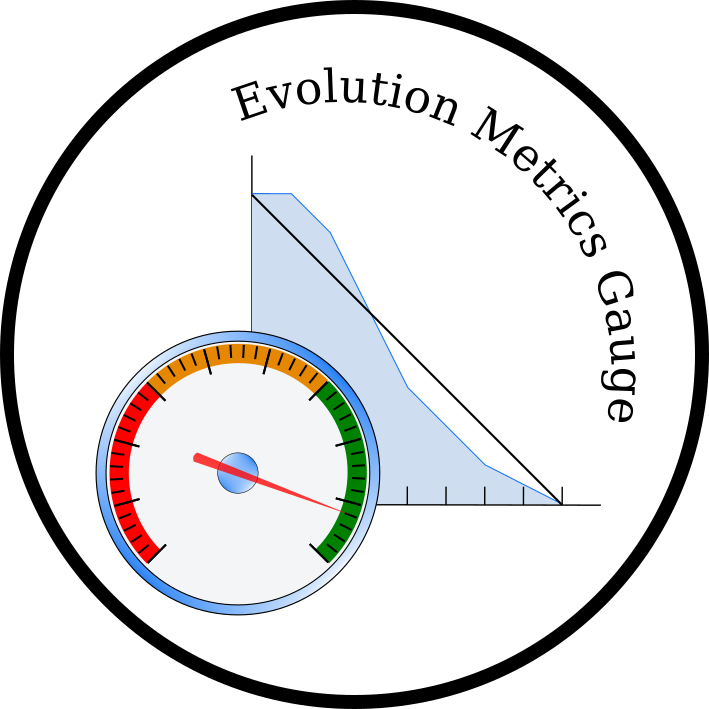
\includegraphics[width=0.5\textwidth]{_LOGOAPP}
	\caption{Logo de Evolution Metrics Gauge}\label{fig:_LOGOAPP}
\end{figure}
\FloatBarrier

En la Fig. \ref{fig:_LOGOAPP} se muestra el logo de la aplicación que se ha mantenido al tratarse este proyecto de una nueva iteración. Éste se compone de un tacómetro que simboliza la medición y un gráfico \textit{burndown} que simboliza la evolución de un proyecto. Lo que se pretende es mostrar la funcionalidad principal de la aplicación: calcular métricas de evolución.


\subsection{Java 11}
% TODO-> actualizar a Java17 si finalmente actualizamos el proyecto
Se ha mantenido la versión utilizada en el proyecto original\cite{TFGPrevio}, Java 11.
Para esta versión, la configuración necesaria de Maven para que el proyecto compile es la siguiente \ruta{pom.xml}:

%Tomcat \footnote{Para desplegar aplicaciones con Java 11 se requiere de la versión 9.0.x de Tomcat} y 
% del proyecto para que Maven compile en la versión 11 de Java:

\begin{minipage}{\linewidth}
{\tiny
\begin{verbatim}[breaklines]
...
<properties>
	<project.build.sourceEncoding>UTF-8</project.build.sourceEncoding>
	<project.reporting.outputEncoding>UTF-8</project.reporting.outputEncoding>
	<java.version>11</java.version>
</properties>
...
<build>
...
	<plugins>
		<plugin>
			<groupId>org.apache.maven.plugins</groupId>
			<artifactId>maven-compiler-plugin</artifactId>
			<configuration>
				<source>${java.version}</source>
				<target>${java.version}</target>
			</configuration>
			<version>3.8.0</version>
		</plugin>
		<plugin>
			<groupId>org.apache.maven.plugins</groupId>
			<artifactId>maven-war-plugin</artifactId>
			<version>3.2.2</version>
		</plugin>
		...
	</plugins>
	...
</build>
...
\end{verbatim}
}
\end{minipage}

Y en Eclipse IDE habría que añadir manualmente el JRE desde la ventana Window/Preferences, como se muestra en la siguiente figura: %Fig. \ref{fig:M5_Eclipse_Java11}.

%TODO imagen con la versión de Java que finalmente adoptemos

% \imagen{M5_Eclipse_Java11}{Añadir Java 11 a Eclipse}

% TODO pendiente de adaptar con la version final de Java adoptada
%De la utilización de Java 11 destacan dos aspectos ya existentes en el proyecto:          
%	\item De la versión 11 se ha utilizado el método \textit{isBlank()} de la clase \textit{String} \footnote{\url{https://docs.oracle.com/en/java/javase/11/docs/api/java.base/java/lang/String.html}}. Se diferencia de \textit{isEmpty()} en que no comprueba la longitud de la cadena y devuelve \textit{true} si es 0. Sino que devuelve \textit{true} si la longitud es 0, o si no es 0 pero todos los caracteres de la cadena son espacios en blanco.
%	\item De la clase \textit{java.util.Optional} \footnote{\url{https://docs.oracle.com/en/java/javase/11/docs/api/java.base/java/util/Optional.html}}, soportada desde la versión 1.8, se utiliza la función \textit{orElseThrow()}, que se soporta desde la versión 10, por tanto habría que buscar una alternativa para pasar a la versión 1.8. La versión 11 trae a esta clase la función \textit{isEmpty()}.
%\end{itemize}
%
%Para saber más sobre las novedades de Java 11 es recomendable leer `\textit{JDK 11 Release Notes}' \cite{oracle_jdk_nodate}. También hay un artículo que explica las principales diferencias entre Java 8 y Java 11 llamado `\textit{De Java 8 a Java 11, ¿aún no te has migrado?}' \cite{del_hoyo_java_2019}.

\subsubsection{Trabajo con streams de Java}

Los \textit{Streams}, presentes en Java desde la versión Java 1.8 son muy útiles ya que facilitan enormemente el procesamiento de grandes colecciones de datos. Estos permiten, usando un predicado, \textbf{filtrar} datos de una colección, \textbf{ordenar} los datos mediante un comparador, \textbf{mapear} o \textbf{reducir} los datos mediante alguna función y \textbf{almacenarlos} en algún tipo de colección mediante un colector. \\ 
Destacan dos funcionalidades, el \textit{mapeo} que asocia cada dato del stream con un nuevo elemento (como el cálculo del cuadrado de cada elemento) y la \textit{reducción} que permite obtener un único resultado a partir del conjunto de datos (como la suma de un conjunto de datos).

Un ejemplo de uso de \textit{streams} en la aplicación:\\
\begin{minipage}{\linewidth}
{\tiny
\begin{verbatim}[breaklines]
...
return gitLabApi.getIssuesApi().getIssuesStream(projectId, new IssueFilter().withState(IssueState.CLOSED))
  .filter(issue -> issue.getCreatedAt() != null && issue.getClosedAt() != null)
  .map(issue -> (int) ((issue.getClosedAt().getTime() - issue.getCreatedAt().getTime()) / (1000 * 60 * 60 * 24 )))
  .collect(Collectors.toList());
...
\end{verbatim}
}
\end{minipage}

En el ejemplo se obtiene de GitLab API un \textit{stream} con las issues cerradas de un proyecto. Este \textit{stream} es filtrado y se obtienen aquellas que tengan fecha de creación y fecha de cierre (\textit{filter}), se calcula de cada \textit{issue} la diferencia en días entre la fecha de creación y la fecha de cierre (\textit{map}), y se recogen los resultados en una lista (\textit{collect}).

%TODO poner otro ejemplo cuando tengamos un acceso a la API de GitHub funcionando

\subsubsection{Interfaces funcionales y funciones lambda de Java}

EN el proyecto también se hace uso de interfaces funcionales y funciones lambda. En la sección anterior ya vemos el uso de dos funciones lambda en el código mostrado (argumentos de las funciones \textit{filter} y \textit{map}).

El paquete \textit{java.util.function} \footnote{\url{https://docs.oracle.com/javase/8/docs/api/java/util/function/package-summary.html}} es soportado por Java desde la versión 1.8. Este paquete permite almacenar funciones en variables. 
\\Las funciones lambda son funciones anónimas con sintaxis \\
\begin{minipage}{\linewidth}
{\tiny
\begin{verbatim}
(parametros) -> {cuerpo funcion lambda}
\end{verbatim}
}
\end{minipage}
que no están declaradas en una clase y pueden ser utilizadas en cualquier parte, pasarse como parámetro a una función y ser almacenadas en variables.
\\Las interfaces funcionales \footnote{\url{https://docs.oracle.com/javase/8/docs/api/java/lang/FunctionalInterface.html}} son interfaces con un único método, que es abstracto, llamado método funcional. Este método permite restringir los tipos de los parámetros y de los valores de retorno de una función lambda.

Estas han sido utilizadas en numerosas ocasiones tanto para los \textit{streams} (como se observa en el código anterior), como en elementos de la interfaz gráfica y otros elementos sensibles a eventos:\\
\begin{minipage}{\linewidth}
{\tiny
\begin{verbatim}[breaklines]
...
closeConnectionButton.addClickListener(event ->  
{
  if(rds.getConnectionType() != EnumConnectionType.NOT_CONNECTED) {
	try {
	  rds.disconnect();
	} catch (RepositoryDataSourceException e) {
		...
	}
  }
  close();
  connectionFormDialog.open();
});
...
\end{verbatim}
}
\end{minipage}

También han sido utilizadas para almacenar funciones en variables, definiendo una interfaz funcional para restringir los tipos parámetros y de los resultados de la función. Un aspecto importante es que las variables que almacenen funciones NO se pueden serializar, por eso la variable \textit{EVAL\_FUNC\_GREATER\_THAN\_Q1} del código siguiente se ha marcado como \textit{transient} dentro de una clase que implementa \textit{Serializable}.

\begin{minipage}{\linewidth}
{\tiny
\begin{verbatim}[breaklines]
...
public interface Metric extends Serializable {
 @FunctionalInterface
 public interface EvaluationFunction {
   EvaluationResult evaluate(IValue value, IValue minValue, IValue maxValue);
 }

 ...
 
 EvaluationResult evaluate(IValue measuredValue);

 EvaluationFunction getEvaluationFunction();
}

...
public abstract class NumericValueMetricTemplate implements Metric {
  ...
  protected transient static final EvaluationFunction EVAL_FUNC_GREATER_THAN_Q1 = 
    (measuredValue, minValue, maxValue) -> 
     {
      try {
        Double value, min;
	    value = ...
	    min = ...
	    if (value > min) return EvaluationResult.GOOD;
	    else if (value.equals(min)) return EvaluationResult.WARNING;
	    else return EvaluationResult.BAD;
	  } catch (Exception e){
	    return EvaluationResult.BAD;
	  }
    };
  ...
}
...
\end{verbatim}
}
\end{minipage}

En el ejemplo anterior muestra la manera en la que las métricas podrían valorarse. La métrica será dada como buena si supera el umbral inferior. Cada métrica podrá usar esta función o implementar una función propia si es necesaria una mayor particularización. Los requisitos definidos en la interfaz funcional son que esa función deberá tener tres argumentos del tipo \textit{IValue} y devolver un resultado del tipo \textit{EvaluationResult}.

\subsection{Maven}

Maven es una herramienta de gestión de proyectos software. Esta herramienta facilita, a partir de un único fichero con extensión \textit{XML} llamado \ruta{pom.xml} \footnote{Project Object Model}:
\begin{itemize}
	\tightlist
	\item La construcción y compilación del proyecto.
	\item La generación de documentación.
	\item La generación de informes.
	\item La gestión de las dependencias del proyecto.
	\item La integración con un sistema de control de versiones como Git, y el trabajo con repositorios remotos como GitLab o GitHub e incluso en repositorios \textit{self-hosted} \footnote{Repositorios almacenados en servidores gestionados por la propia empresa o equipo que desarrolla el software}.
	\item La generación y distribución de \textit{releases}.
\end{itemize}
Maven puede crear la estructura de directorios del proyecto, administrar las dependencias y descargar las librerías necesarias. Además, es compatible con la mayoría de IDEs \footnote{Integrated Development Environment - Entorno de desarrollo integrado}. Por ejemplo, en este proyecto se ha trabajado sobre Eclipse IDE, el cual tiene muy buena integración con Maven, como se puede observar en la Fig. \ref{fig:M5_Eclipse_Maven}.

\imagen{M5_Eclipse_Maven}{Integración de Maven con Eclipse}

También permite el uso de arquetipos, que son patrones o plantillas que se aplican en la infraestructura del proyecto.

Aunque puede resultar difícil configurar correctamente Maven a través del archivo de configuración, debido sobre todo al buen número de herramientas a configurar en él, una vez configurado, nos ahorra mucho tiempo y nos permite centrarnos en el desarrollo de funcionalidad.

\subsection{Sistema de control de versiones}

Se ha utilizado Git para el desarrollo del proyecto para el control de versiones y se ha utilizado GitHub como repositorio remoto. 

GitHub no sólo ha permitido el almacenamiento del código del proyecto si no que también ha permitido el seguimiento y colaboración alumno-tutor gracias a las herramientas que proporciona. Además, utilizando ZenHub (que se puede integrar en el propio GitHub) se ha llevado a cabo la gestión de las tareas (\textit{issues}) del proyecto. Como se puede observar en la Fig. \ref{fig:M5_GitHub-ZenHub_board}.

\imagen{M5_GitHub-ZenHub_board}{Tablero de Scrum en ZenHub integrado en GitHub}

Es posible configurar Eclipse y Maven para trabajar con Git. Sin embargo, debido a la costumbre de uso directamente en consola del alumno, se ha optado por el uso de GitBash tal y como se muestra en la Fig. \ref{fig:M5_GitBash}.

\imagen{M5_GitBash}{Consola para Git de Windows GitBash}

\subsection{Logging}

% TODO
\capitulo{6}{Trabajos relacionados}

Se van a comentar diferentes aplicaciones con funcionalidad similar al presente proyecto y compararlas con él, cabe destacar que aunque hay similitudes, no se ha encontrado en el mercado ninguna solución con las características de framework de medición y extensibilidad a diferentes forjas que tiene el presente proyecto.

\section{Criticality-Score}
Se trata de una aplicación de consola escrita en Python por miembros del Open Source Security Foundation (OpenSSF) \footnote{Open Software Security Foundation:  \url{https://openssf.org/} - \url{https://github.com/ossf}} que tiene como objetivo puntuar con una puntuación crítica a  todos los proyectos \textit{open source} posibles para así ver de qué proyectos depende más la comunidad de desarrolladores de todo el mundo y poder así aumentar la seguridad de dichos proyectos.\\

Podemos encontrar la aplicación en:\\
\url{https://github.com/ossf/criticality_score}


La puntuación de criticidad de un proyecto define la influencia y la importancia de un proyecto. Es un número entre 0 (menos crítico) y 1 (más crítico). Se basa en el algoritmo de medida de la criticidad de Rob Pike  \footnote{Quantifying Criticality by Rob Pike  \url{https://github.com/ossf/criticality_score/blob/main/Quantifying_criticality_algorithm.pdf}} que utiliza una serie de parámetros como las fechas de creación y actualización del proyecto, el número de colaboradores o el número de \textit{issues} cerradas entre otros. Una vez se tienen los parámetros obtenidos de los repositorios, se opera con ellos utilizando el algoritmo y se obtiene una puntuación (el \textit{criticality-score}.

En este proyecto se trabaja con repositorios de GitHub y GitLab utilizando API-token como en el presente proyecto, sin embargo no es extensible a otras forjas de repositorios. Tampoco se tiene umbrales para los parámetros y no podemos valorar con esta herramienta si los valores obtenidos para calcular el \textit{criticality-score} son apropiados o no.


\section{Agile-Metrics}
Agile Metrics es un recopilador de datos de KPI del proceso de desarrollo de software. Recopila mediciones de los productores (forjas de repositorios), crea métricas y las envía a los consumidores (procesadores de datos los datos de métricas para proporcionar un procesamiento posterior, por ejemplo, visualización. Sólo está soportado ElasticSearch). Soporta tres productores o forja, BitBucket, JIRA Software Server y SonarQube. Trabaja con diferentes métricas dependiendo de donde esté alojado el repositorio, por ejemplo con BitBucket sólo calcula los commits diarios por autor, proyecto o repositorio mientras que con JIRA Software Server calcula 13 métricas entre las que podemos nombrar el ratio de \textit{bugs} o el volumen de issues.\\

La idea tras la cual nace esta aplicación escrita en Java es muy similar a la del proyecto actual, pero está enfocado a necesidades más concretas pues no trabaja con las forjas de repositorios más comunes (GitHub y GitLab) y además no unifica las métricas calculadas si no que es dependiente de la forja con la que se trabaje en ese momento.

Podemos encontrar la aplicación en:\\
\url{https://github.com/DaGrisa/agile-metrics#consumer}



\section{Activity-API}
Se trata de una aplicación desarrollada también en el entorno de un trabajo fin de carrera, similar en funcionalidad al proyecto actual. Está implementada como aplicación de escritorio en lenguaje Java y fue usado como inspiración en algunos aspectos de modelo para la primera versión inicial\cite{TFGPrevio} de este proyecto. \\
Se trata de una aplicación alojada en GitHub\footnote{\url{https://github.com/dba0010/Activiti-Api}} y que se puede obtener y ejecutar pues es opensource. Esta aplicación trabaja sólo con GitHub pero tiene implementada una versión de un framework que permitiría la extensibilidad a otras forjas de manera similar a este proyecto.\\
Activity-API permite evaluar un proyecto o comparar sólo dos entre ellos (una clara desventaja frente a este proyecto que permite añadir proyectos de forma ilimitada para compararlos). De forma similar a este proyecto muestra los resultados en forma de tabla y también trabaja con umbrales (definidos a partir de unas estadísticas obtenidas de un conjunto de datos obtenidos a partir de TFGs y publicado en GitHub \footnote{\url{https://github.com/clopezno/clopezno.github.io/blob/master/agile_practices_experiment/DataSet_EvolutionSoftwareMetrics_FYP.csv}}  para valorar las métricas muestra los valores obtenidos para las métricas y si entran o no en los umbrales por colores como se puede ver en la siguiente figura:

\begin{figure}[!h]
	\centering
	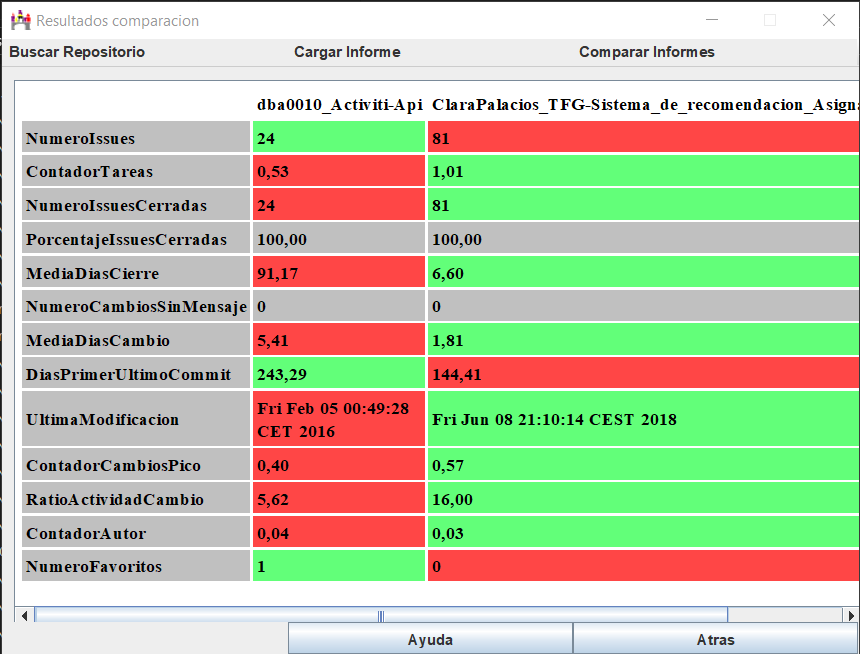
\includegraphics[width=0.65\textwidth]{M6_AA_Comparativa}
	\caption{Comparación de dos proyectos utilizando Activiti-Api}\label{fig:M6_AA_Comparativa}
\end{figure}
\FloatBarrier

Además permite la exportación de los resultados como en este proyecto aunque luego no permite importarlos.


\section{Tablas comparativas}

Podemos comparar diferentes características de las herramientas con el proyecto, comparando si son extensibles en cuanto a forjas de repositorios o métricas o no entre otras características.\\

\newpage
Como podemos ver en las tablas anteriores, el proyecto actual destaca claramente en cuanto a extensibilidad y capacidad de configuración, se pueden añadir más forjas de repositorios y nuevas métricas mientras que en el resto de herramientas es más complicado ya que están acopladas a las integraciones que tienen con las forjas de repositorios con las que trabajan.\\
Además, cabe destacar que aunque las herramientas también comparan repositorios entre sí como hacemos en este proyecto, no permiten trabajar con umbrales de las mismas con lo que se pierde mucha perspectiva y el usuario no sabe si los valores de dichas métricas son aceptables (o incluso lógicos) o no.\\

\tablaSmall{Tabla comparativa de herramientas, forjas}{l c c c c}{comparativa1}
{ \multicolumn{1}{l}{Herramientas} & Forjas & Extensible & OpenSource & Actualizado\\}{ 
Comparador-de-métricas & 2 & X & X & 2022\\
Criticality-Score & 2 & & X & 2022\\
Agile-Metrics & 3 & & X & 2018\\
Activity-API & 1 & & X & 2016\\
} 


\tablaSmall{Tabla comparativa de herramientas, métricas}{l c c c c}{comparativa1}
{ \multicolumn{1}{l}{Herramientas} & Métricas & Extensible & Umbrales & Configurables\\}{ 
Comparador-de-métricas & 13 & X & X & X\\
Criticality-Score & 1 & & &\\
Agile-Metrics & 3-10 & & &\\
Activity-API & 13 & & X & X\\
} 

\newpage
\subsubsection{Mantenibilidad y extensibilidad}

\textit{Evolution Metrics Gauge} ha preparado un framework para poder extenderse a otras forjas de repositorios, se implementó originalmente sólo trabajando con Gitlab y se ha extendido en este proyecto añadiendo GitHub a las forjas soportadas. Ninguna de las herramientas con las que hemos comparado este proyecto permite esta extensibilidad e incluyen demasiadas dependencias con las API de las forjas con las que trabajan.

En cuanto a la extensibilidad referente a las métricas, sólo en algunos se podría trabajar con más métricas pero ninguno trabaja con las mismas métricas como se hace en este proyecto gracias a la implementación del framework de medición que hemos visto anteriormente.

Por todo lo anterior, podemos decir que en la industria no existe actualmente ninguna solución estandarizada y que sea extensible para medir y analizar las métricas de evolución de los repositorios software por lo que este proyecto da una solución que hasta ahora no existe en el mercado, por lo que puede aportar gran valor.\\

Como se ha explicado anteriormente, la funcionalidad de este proyecto se puede ampliar tal y como se ha hecho en este TFG a otras forjas como BitBucket y añadir nuevas métricas (siempre que todas las forjas provean de la información necesaria para calcularas a través de sus API), pudiendo llegar a ser un estandard que cubra cualquiera de las necesidades que pueda tener un usuario que necesite analizar métricas de evolución de sus repositorios software.

\newpage
\section{Otros trabajos relacionados}
\begin{itemize}
	\item \textbf{Soporte de Métricas con Independencia del Lenguaje para la Inferencia de Refactorizaciones}. Base sobre la que se ha realizó la construcción del subsistema ``motor de métricas'' y sobre la que se han implementado las nuevas funcionalidades en este proyecto. Se puede consultar más información al respecto en la sección \ref{sect:3_3_3_FrameworkMedicion} en el apartado `Framework de medición'.
	
	\item \textbf{Software Project Assessment in the Course of Evolution -  Jacek Ratzinger}.De este trabajo de donde se obtuvieron las métricas de control con las que trabajaba \textit{Evolution Metrics Gauge} inicialmente (en este proyecto se han ampliado con métricas referentes a Integración y Despliegue Coninuo o CICD). Hay una explicación detallada en el apartado \ref{sect:3_3_2_MetricasControl} en el apartado `Métricas de control: medición de la evolución o proceso de software'.

	\item \textbf{Key Metrics to Track and Drive Your Agile Devops Maturity}\cite{KeyDevOpsMetrics}. De este artículo se han tomado ideas y se ha visto la necesidad de añadir métricas relacionadas con DevOps, es decir métricas referentes a Integración y Despliegue Coninuo o CICD. De esta necesidad han surgido las 5 métricas añadidas al proyecto, ver \ref{sect:3_3_2_MetricasControl}.
\end{itemize}
\capitulo{7}{Conclusiones y Líneas de trabajo futuras}

A continuación se van a exponer las conclusiones obtenidas tras la realización del trabajo y las posibles líneas de trabajo futuras con las que se podría seguir mejorando la funcionalidad del proyecto.

\section{Conclusiones}
Las conclusiones obtenidas tras las realización del proyecto podríamos dividirlas en dos grupos, unas conclusiones con un carácter más teórico basadas en la consecución de los objetivos planteados al inicio del proyecto y otras relacionadas con las herramientas utilizadas con un carácter más técnico.

En cuanto a las primeras, se ha concluido que:

\begin{itemize}
	\item Se ha completado el objetivo de integrar \textit{GitHub} con la aplicación, haciendo posible trabajar con repositorios alojados tanto en \textit{GitLab} como en \textit{GitHub}.
	\item Se han añadido cinco nuevas métricas relacionadas con la integración y despliegue continuos, un tipo de métricas con las que aún no se trabajaba.
	\item Se ha probado con repositorios reales que tanto la funcionalidad previa como la nueva se lleva a cabo correctamente y que la aplicación cumple con el objetivo de poder comparar repositorios calculando sus métricas de evolución. Gracias a esto se ha podido crear un perfi de métricas con los TFGs presentados en los pasados años que se puede encontrar en: \\url{}.
	\item Gracias al estudio y comprensión de las diferentes métricas, así como la implementación de nuevas y el mantenimiento de las ya existentes, podemos confirmar las métricas de evolución son tan importantes como las métricas de producto a pesar de que actualmente están relegadas a un segundo plano respecto a las de producto. Estudiar ambos tipos de métricas es clave para obtener un software de calidad, si el proceso de creación de software no se cuida y sólo se vela por el producto final, éste acabará teniendo peor calidad. 
	\item La extensibilidad es un factor clave a la hora de mantener y mejorar el software. En este proyecto ha sido clave la estructura como \textit{framework} que permite la adición de nuevas forjas de repositorios así como nuevas métricas para poder integrar \textit{GitHub} y añadir las nuevas métricas.
	\item Los repositorios y las forjas de repositorios facilitan el proceso de desarrollo del software y nos dan herramientas para monitorizarlo, evaluarlo y si estimamos oportuno, mejorarlo si detectamos problemas gracias a las métricas y sus umbrales.
\end{itemize}

Y por último, relativas a las herramientas utilizadas, se ha concluido que:

\begin{itemize}
	\item La integración y despliegue continuo, por medio de la realización de tests junto a la revisión automática de calidad de código nos ayuda a detectar errores, lo que permite corregirlos antes incluso de subir nuestro código al repositorio remoto donde lo estemos alojando. \textit{GitHub} por medio de \textit{GitHub actions} nos proporciona una magnífica herramienta que nos permite establecer flujos de acciones o \textit{jobs} a ejecutar al subir código al repositorio remoto. Esto nos permite mantener un flujo automatizado que nos ayuda a tener una versión de nuestra aplicación actualizada desplegada en todo momento. 
	\item Maven es un gran gestor de proyectos software escritos en \textit{Java} y ayuda a trabajar con los mismos en todas sus fases, facilitando la configuración necesaria para integrar todas las herramientas y \textit{plugins} necesarios.
	\item \textit{Vaadin} es un \textbf{framework} que nos permite crear aplicaciones web modernas utilizando Java lo cual es una ventaja si no estamos familiarizados con otros lenguajes como \textit{JavaScript} o necesitamos trabajar con \textit{Java}. Sin embargo, tiene un gran coste de aprendizaje ya que al tener toda la funcionalidad de la interfaz y la lógica unidas, puede dificultar la comprensión y mantenibilidad del código. Además, cabe indicar que es poco personalizable en comparación con otras alternativas que están liderando actualmente el desarrollo web como pueden ser \textit{Angular}, \textit{React} o \textit{Vue}, que además tienen una curva de aprendizaje más suave y una comunidad de usuarios mucho mayor.
\end{itemize}

\newpage
\section{Líneas de trabajo futuras}
Algunos de los aspectos en los que se podría seguir trabajando para evolucionar y mejorar el proyecto son:\\
\begin{itemize}
	\item Extender la funcionalidad a otras métricas de evolución
	\item Extender a otras forjas de repositorios como \textit{Bitbucket}, realizando una integración y adaptaciones de la interfaz gráfica similares a las realizadas para \textit{GitHub} en este proyecto.
	\item Soporte de entorno multisesión y gestión de usuarios con un sistema de autenticación ya sea propio contra una base de datos o bien utilizando alguna solución externa como \textit{Firebase Authentication}.
	\item Realizar un histórico de mediciones y almacenarlo en una base de datos.
	\item Almacenamiento de perfiles de métricas en base de datos.
	\item Mejorar la interfaz web para sea adaptativa a los diferentes tamaños de pantalla (\textit{responsive}).
	\item Internacionalizar la aplicación soportando diferentes idiomas.
	\item Mejoras de usabilidad como permitir borrar, evaluar o actualizar varios repositorios al mismo tiempo.
	\item En repositorios grandes las consultas a las \textit{APIs} de las forjas de repositorios pueden ser muy largas debido a que tienen acceso limitado. Este problema se aprecia principalmente en repositorios grandes alojados en \textit{GitLab}. Se podría evitar que la aplicación se quede esperando mientras finalizan dichas peticiones si se externalizan en un micro-servicio las consultas a las \textit{APIs} de las forjas.
	
\end{itemize}


\bibliographystyle{plain}
\bibliography{bibliografia}

\end{document}
